\documentclass{article}
\usepackage[english]{babel}
\usepackage{graphicx} % Required for inserting images

%\usepackage[francais]{babel}
% \usepackage[latin1]{inputenc}
\usepackage{float}
\usepackage{pgfplotstable}
\pgfplotsset{compat=1.17}
\usepackage{graphicx}
\usepackage{pdfpages}
\usepackage{float}
\usepackage{calc,xcolor}
\usepackage{tabularx}
\usepackage{wrapfig}
\usepackage{caption}
\usepackage{amsmath}
\usepackage{braket}

\usepackage[export]{adjustbox}

\usepackage[colorlinks=true]{hyperref}
%\usepackage{dcolumn}
%\usepackage{bm}
\usepackage{titlesec}
\usepackage{pgfplots}
\usepackage{booktabs, multirow}
\usepackage{soul}
\pgfplotsset{compat=1.18} 
\usepackage{longtable}
\usepackage{csvsimple,longtable,booktabs, pgfplots}
\usepackage{siunitx}
\usepackage{makecell}
\pgfplotsset{compat=1.18} 
\usepackage{multirow}

\frenchspacing 
\setlength{\paperwidth}{21cm}
\setlength{\paperheight}{29.7cm} 
\setlength{\textwidth}{16.5cm}
\setlength{\textheight}{24.5cm} 
\setlength{\oddsidemargin}{0.5cm}
\setlength{\evensidemargin}{-0.5cm} 
\setlength{\marginparwidth}{0cm}
\setlength{\leftmargin}{0cm} 
\setlength{\topmargin}{0cm}
\setlength{\headsep}{1cm} 
\setlength{\footskip}{1.5cm}
\setlength{\voffset}{-3cm} 
\setlength{\hoffset}{-0.5cm}

\title{Ageing Pipes Analysis}
\author{Yohan VERROQUET}
\date{November 2025}


\begin{document}
\maketitle
\newpage
\tableofcontents
\listoffigures           % Liste des figures
\listoftables            % Liste des tableaux
\newpage



\section{Introduction}
Ageing of buried drinking-water pipes made of unplasticized poly(vinyl chloride) (uPVC) is a critical issue for water distribution networks. Over time, uPVC pipes undergo physical and chemical changes that can lead to a loss of elasticity, embrittlement, and ultimately mechanical failure. Understanding how ageing affects the material properties is therefore essential for improving failure prediction and enabling reliable non-destructive evaluation (NDE) techniques.

In this study, several uPVC pipe sections originating from different locations, manufacturers, and installation years were collected after excavation. To reproduce and accelerate ageing under controlled conditions, samples were placed in a oven at 70 °C for four different durations:

0 days (reference condition),

4 days,

1 week,

2 weeks.

After thermal ageing, each set of samples underwent a series of complementary characterization tests:

Density measurements,

Differential Scanning Calorimetry (DSC) to determine the glass transition temperature and enthalpy of relaxation,

Tensile tests to quantify changes in Young’s modulus, yield behaviour, and fracture properties,

Nonlinear ultrasonic wave-mixing experiments, aiming to evaluate the potential of nonlinear acoustics as a non-destructive technique of ageing and mechanical degradation.

The overall objective is to establish correlations between nonlinear ultrasonic wave-mixing responses and mechanical ageing properties.
\begin{table}[h!]
\centering
\caption{Informations about collected pipes}
\begin{tabularx}{\textwidth}{|l|X|X|X|X|}
\hline
\textbf{Pipe} & \textbf{DYKA 2003} & \textbf{WAVIN KIWA 1987} & \textbf{WAVIN APOLLO BIAX} & \textbf{WAVIN 1980} \\
\hline
Date of production & 25/01/2003 & 18/03/1987 & 24/05/2001 & January 1980 \\
\hline
Date of installation & ? & 1987 & 2002 & 1980 \\
\hline
Date of excavation &  & 03/10/2025 & May 2025 & 2025 \\
\hline
Dimensions & 160*4,7 mm & 160*4 mm & 160 mm & 200*4 mm \\
\hline
Manufacturer & DYKA & WAVIN & WAVIN & WAVIN \\
\hline
Other specifications & KIWA PVC 0,75MPa & KIWA K.49; 0,63MPa; 178-01 PL C. & PVC-U Biaxial-320 KIWA BRL-K565 SOR41 PN10 125-49 & PVC KIWA K 49 KG CM2 9 7 1-80 125 38 \\
\hline
Location & Hoofddorp/ Rijnlanderweg & Mounleane 43, Uretep &  & CCF LWD \\
\hline
Reason for excavation & Upgrading the distribution network & Reconstruction of a nearby bridge/network & Reconstruction of network & Improvement of connection \\
\hline
Observations &  & PVC easily breaks, indicated as bad quality by crew &  & Made for nominal pressure 6 bar, pipe is completely brown discolored on outside \\
\hline
Soil type & Klei &  &  & sand fill \\
\hline
\end{tabularx}
\end{table}

\section{Density}
Density measurements were performed on samples extracted from each pipe with the Density kit.

\begin{figure}[H][H]
    \centering
    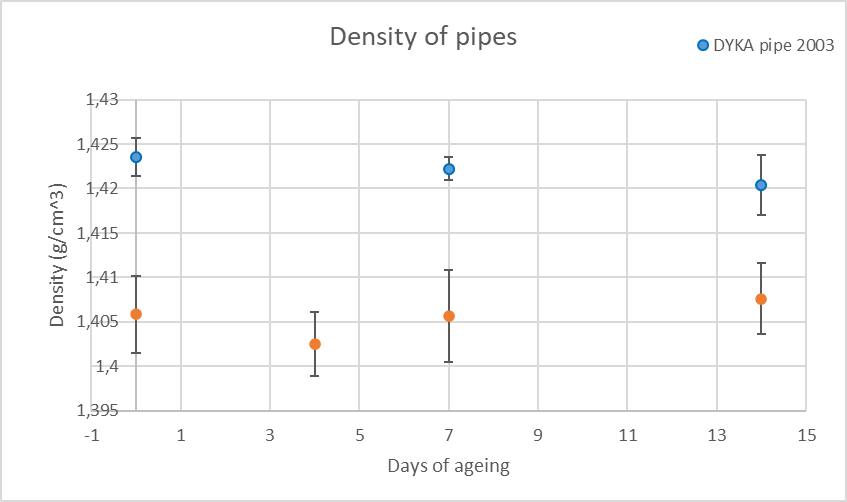
\includegraphics[width=0.75\linewidth]{density_graph.png}
    \caption{Density of pipes}
    \label{fig:density_graph}
\end{figure}

\section{DSC analysis}
Differential Scanning Calorimetry (DSC) was used to quantify the thermal transitions of uPVC, with particular attention to the glass transition temperature (Tg) and the enthalpy of relaxation.
\subsection{DYKA 2003 pipe}
\subsubsection{0 day ageing}

\begin{figure}[H]
    \centering
    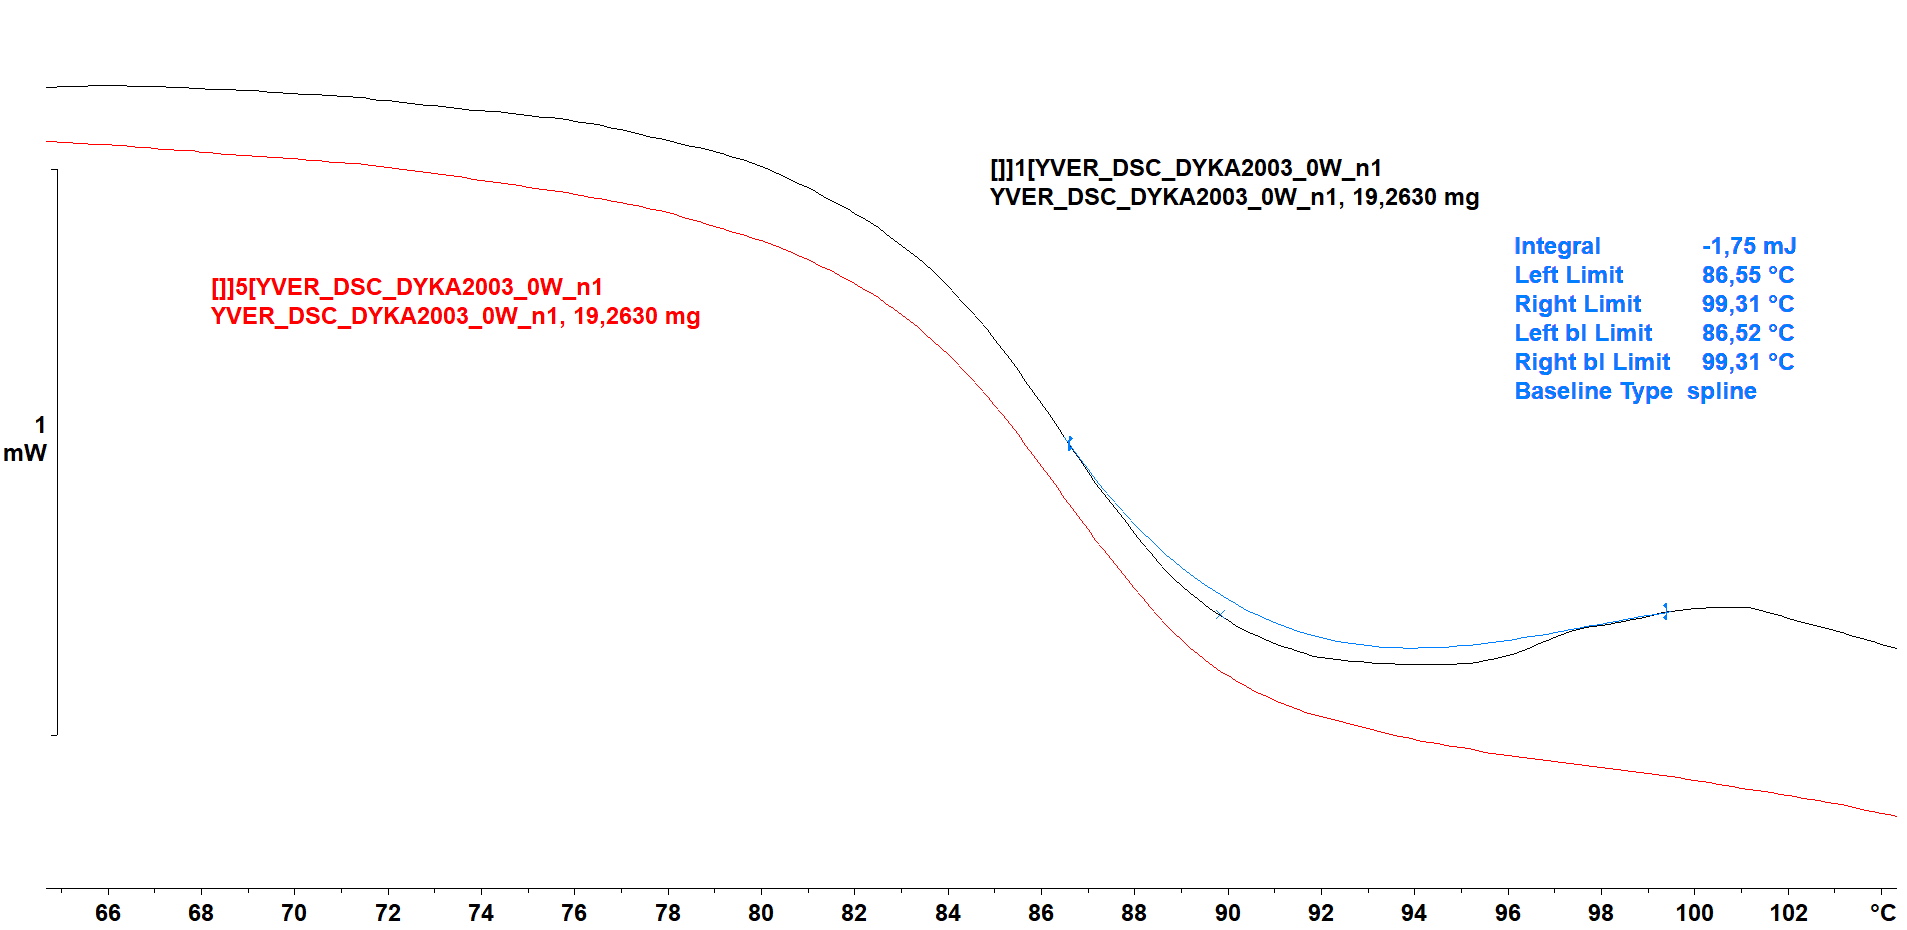
\includegraphics[width=0.75\linewidth]{DYKA2003_0d_n1.png}
    \caption{Endothermic peak of DYKA 2003, 0 day ageing, n°1}
    \label{fig:dyka2003_0d_n1}
\end{figure}

\begin{figure}[H]
    \centering
    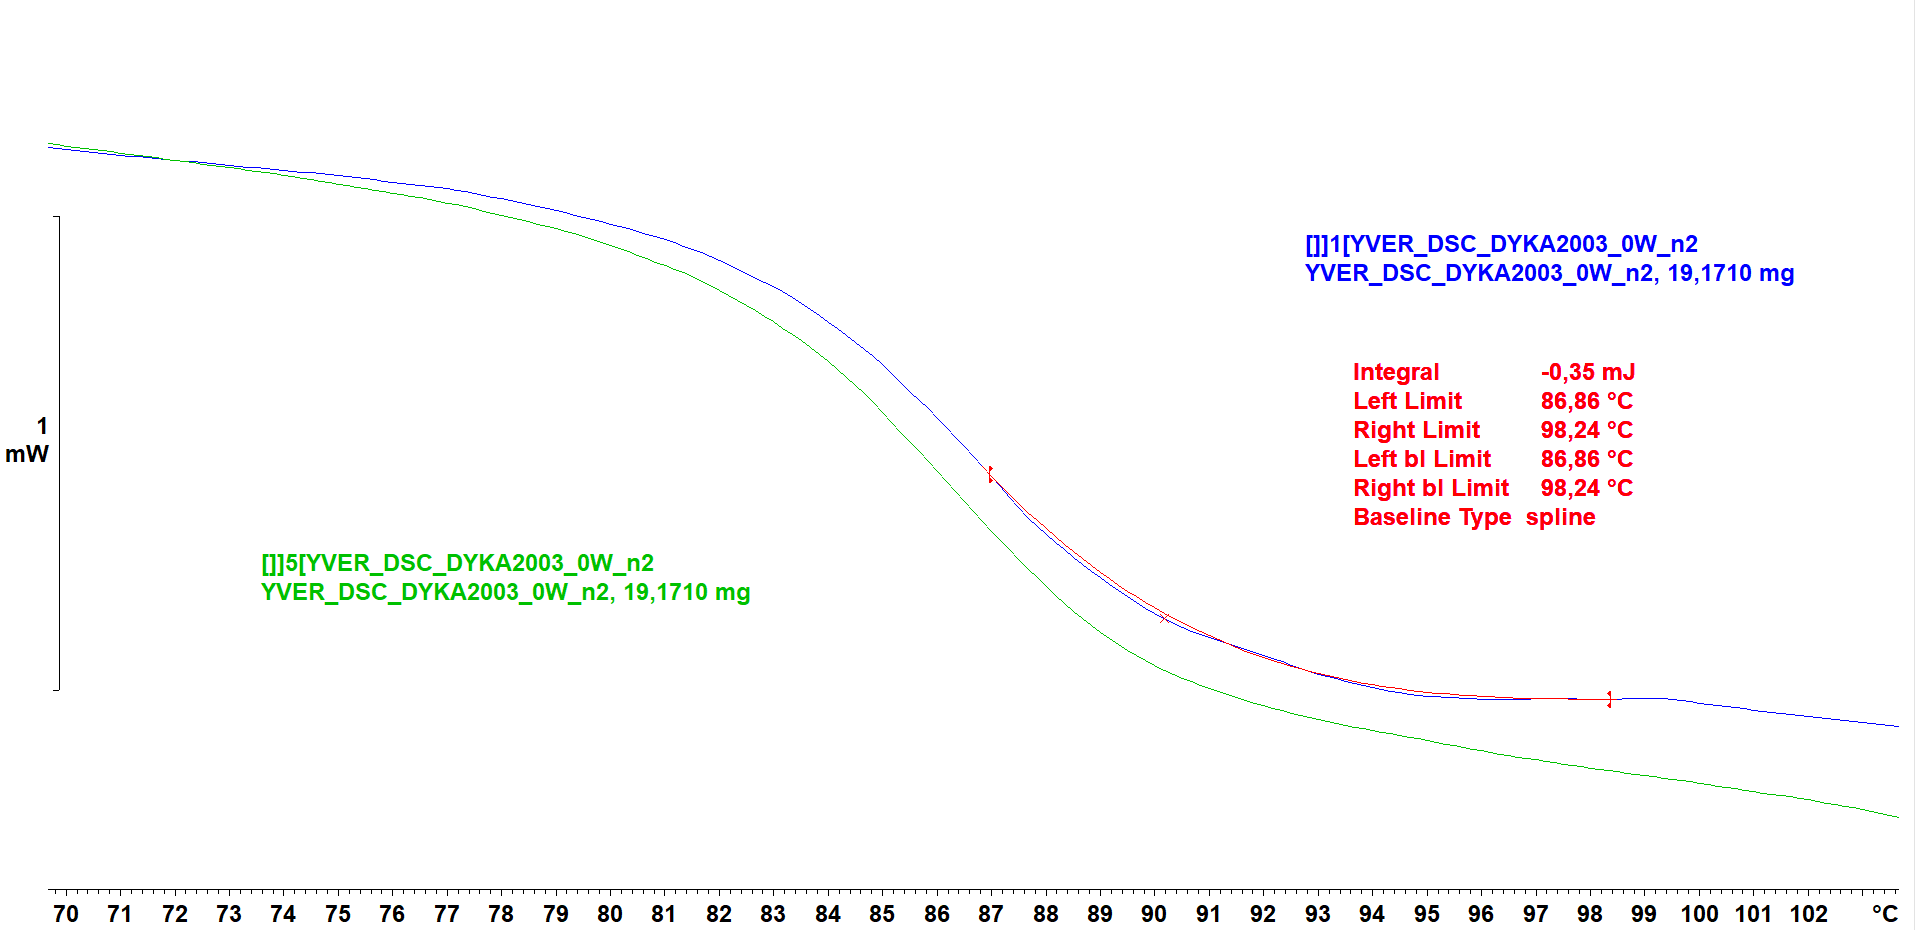
\includegraphics[width=0.75\linewidth]{DYKA2003_0d_n2.png}
    \caption{Endothermic peak of DYKA 2003, 0 day ageing, n°2}
    \label{fig:dyka2003_0d_n2}
\end{figure}

\begin{figure}[H]
    \centering
    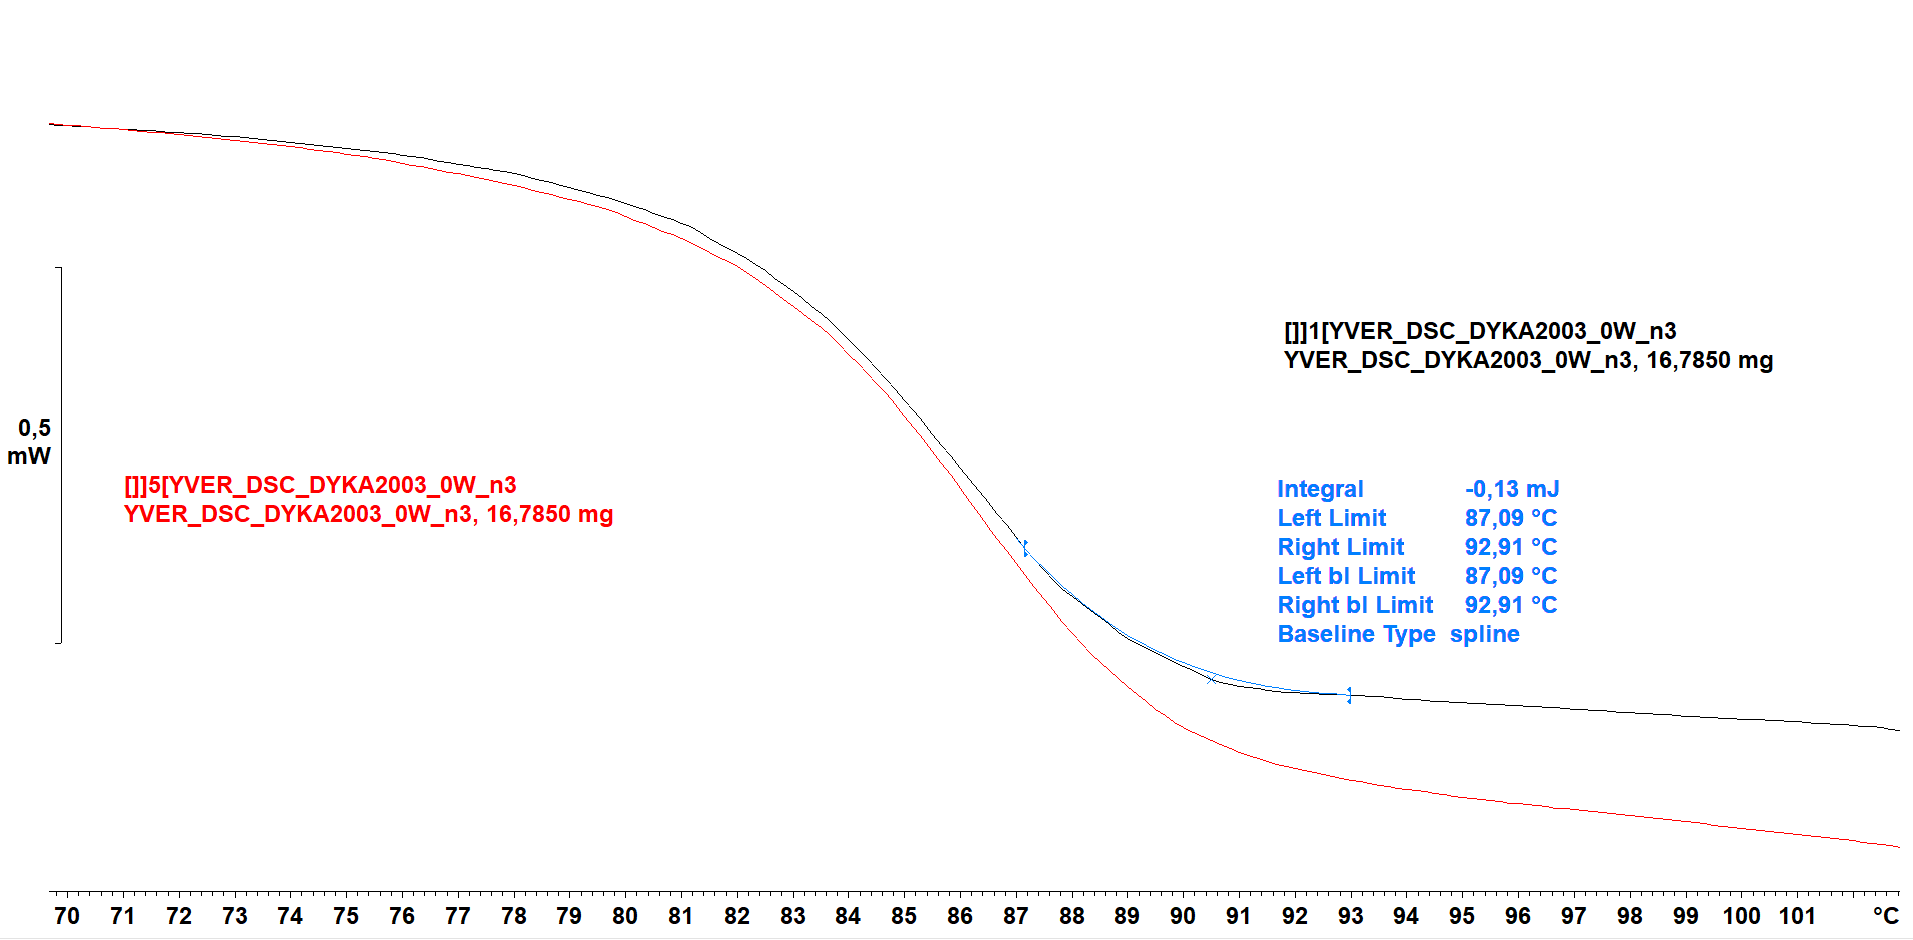
\includegraphics[width=0.75\linewidth]{DYKA2003_0d_n3.png}
    \caption{Endothermic peak of DYKA 2003, 0 day ageing, n°3}
    \label{fig:dyka2003_0d_n3}
\end{figure}

\begin{figure}[H]
    \centering
    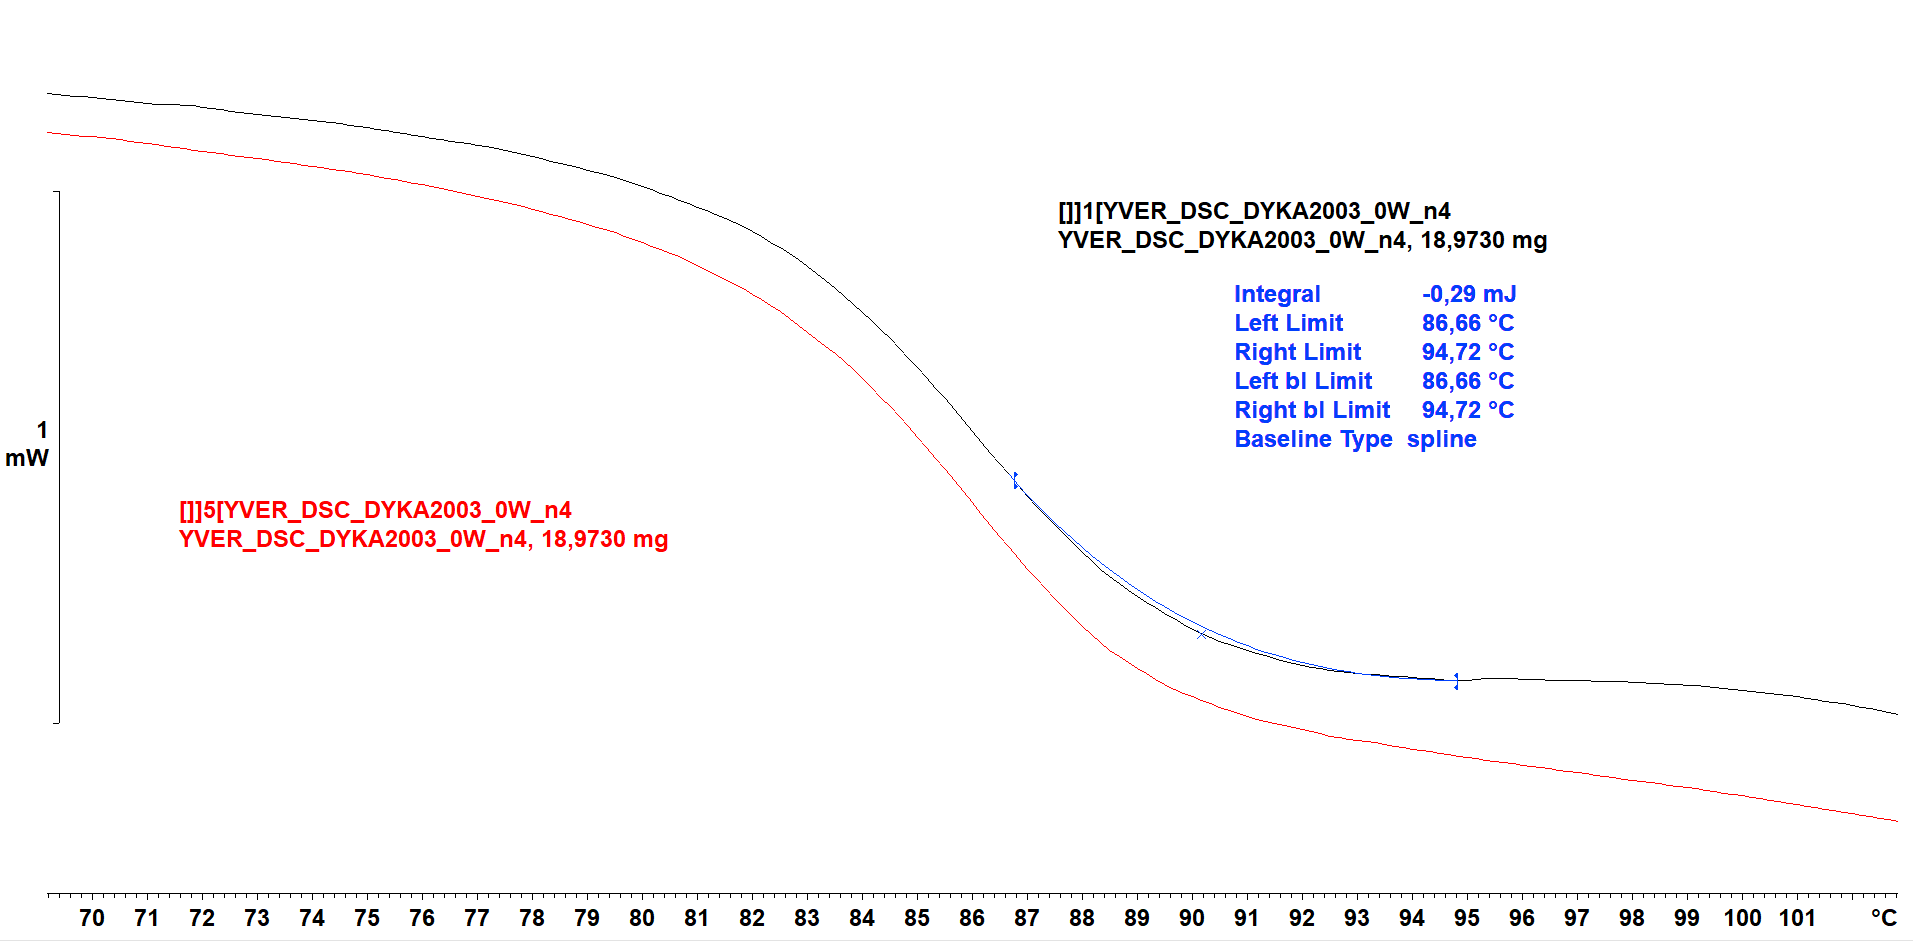
\includegraphics[width=0.75\linewidth]{DYKA2003_0d_n4.png}
    \caption{Endothermic peak of DYKA 2003, 0 day ageing, n°4}
    \label{fig:dyka2003_0d_n4}
\end{figure}

\subsubsection{1 week ageing}
\begin{figure}[H]
    \centering
    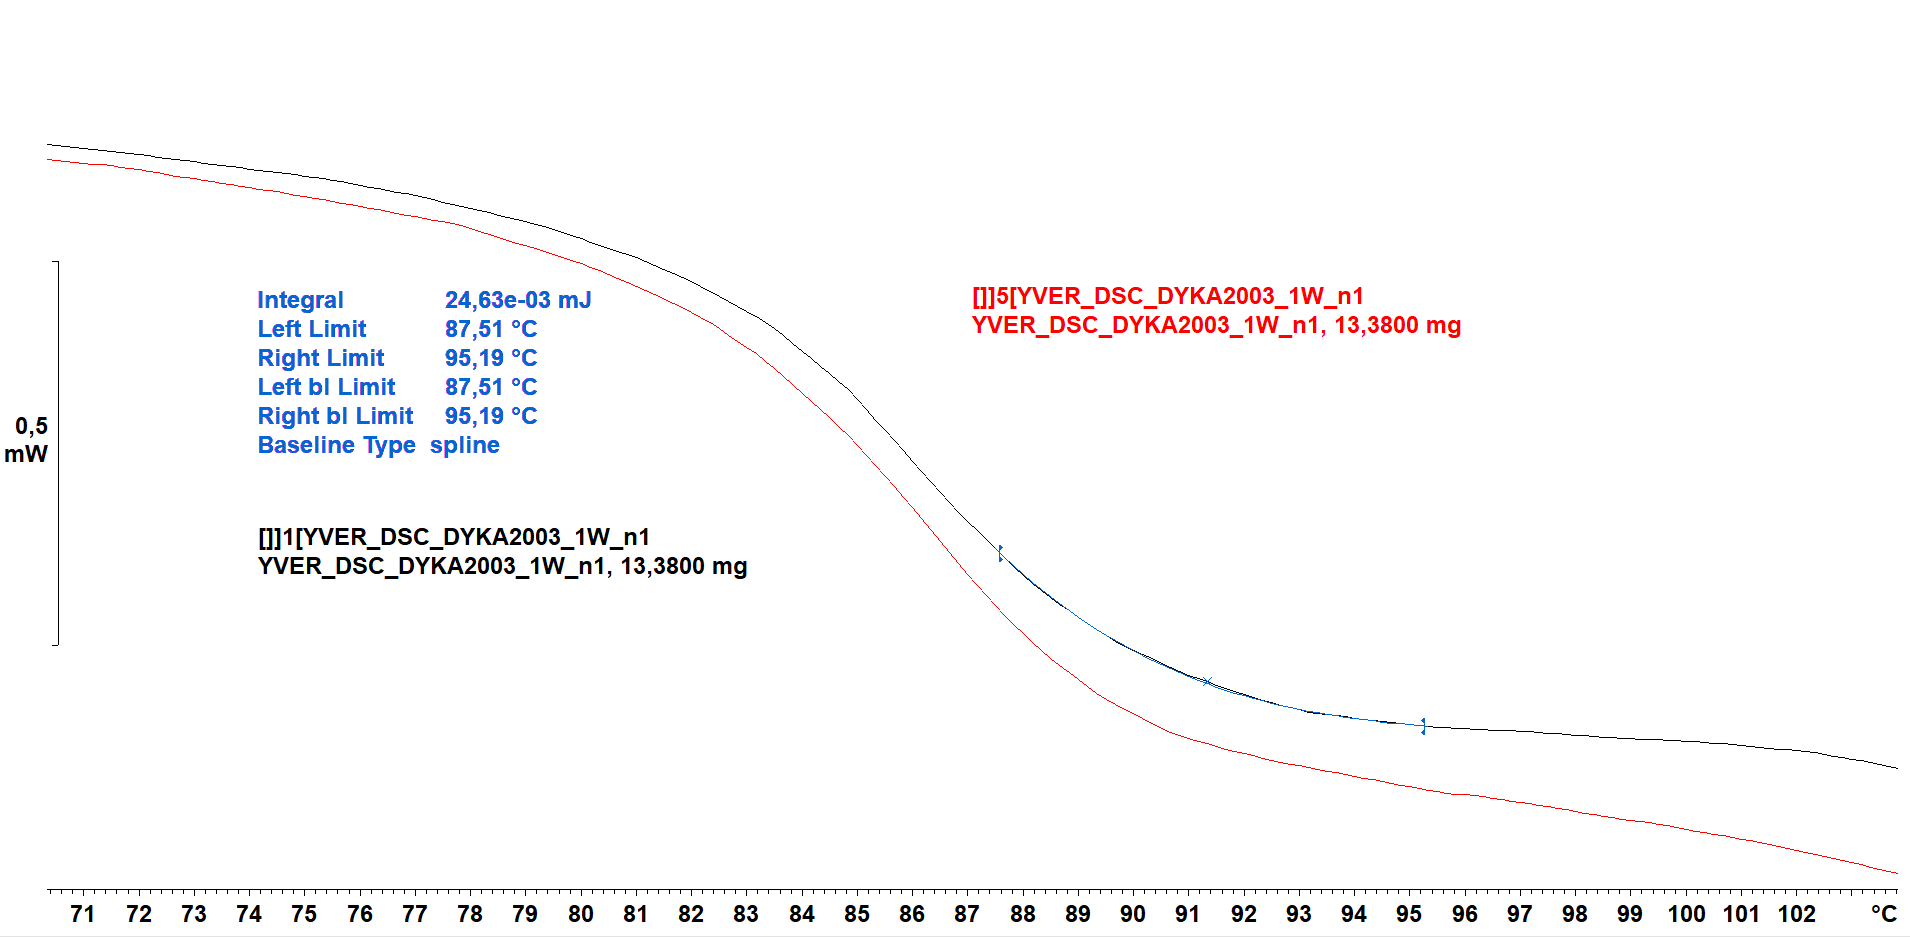
\includegraphics[width=0.75\linewidth]{DYKA2003_1w_n1.png}
    \caption{Endothermic peak of DYKA 2003, 1 week ageing, n°1}
    \label{fig:dyka2003_1w_n1}
\end{figure}

\begin{figure}[H]
    \centering
    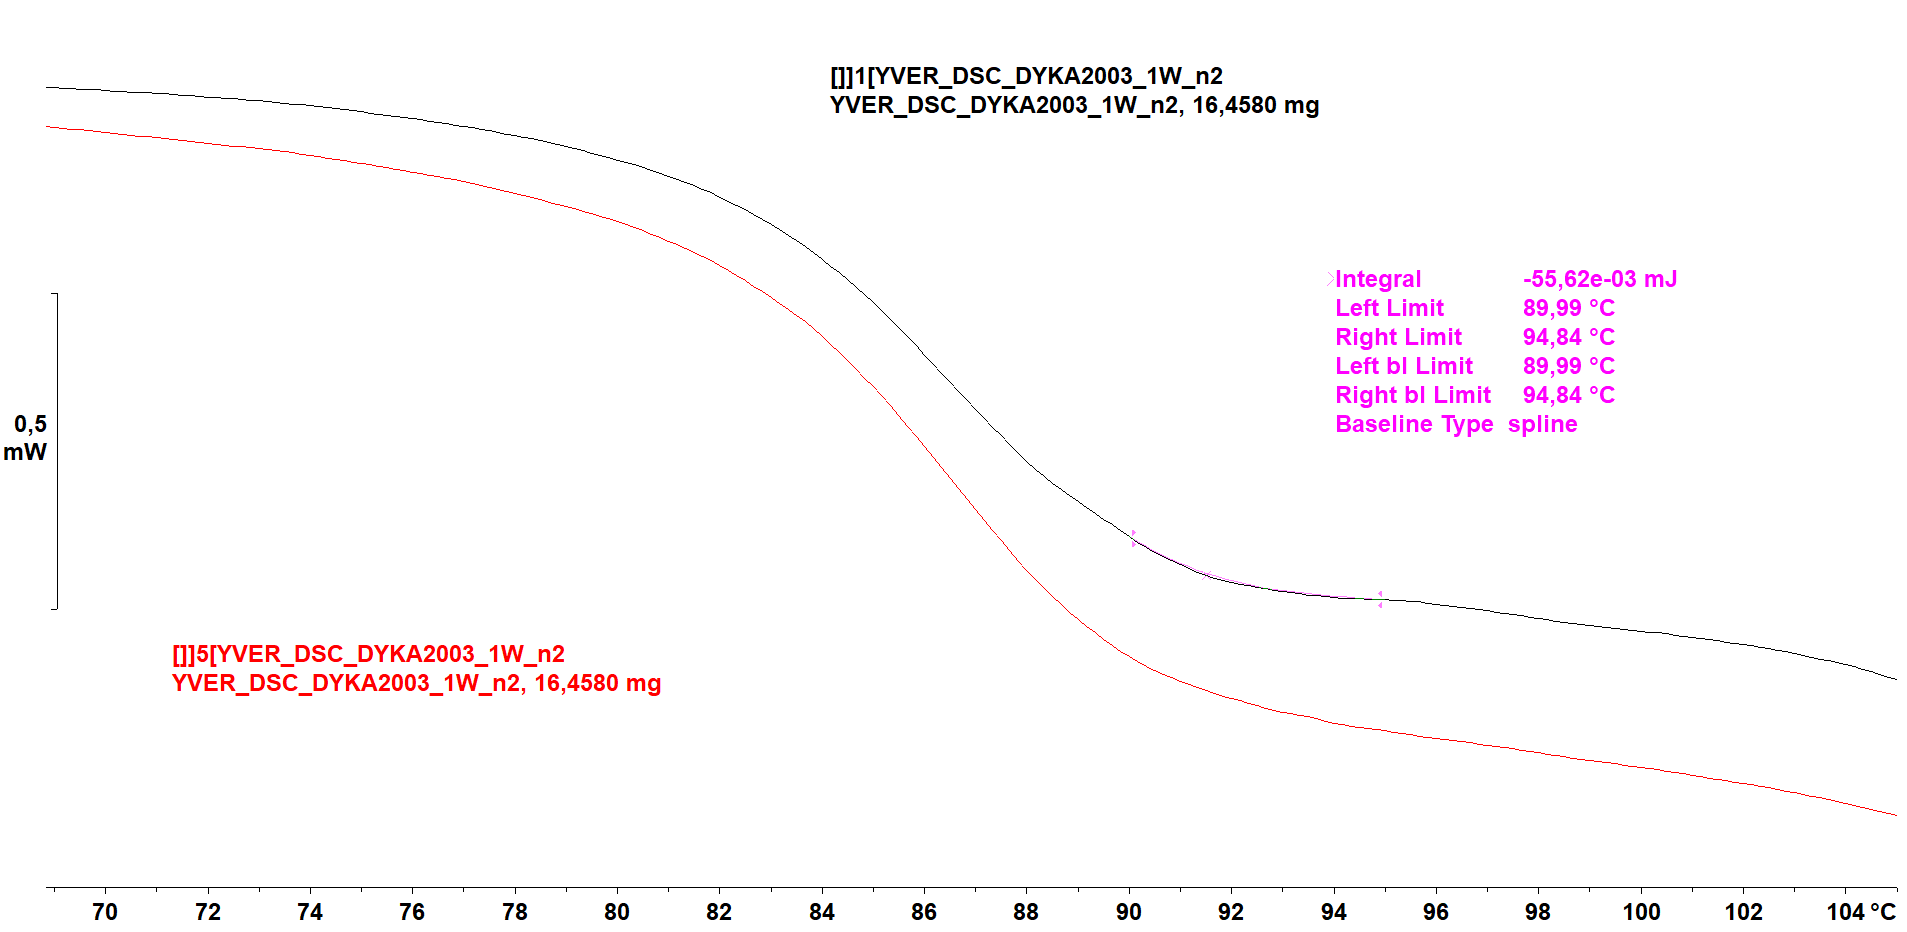
\includegraphics[width=0.75\linewidth]{DYKA2003_1w_n2.png}
    \caption{Endothermic peak of DYKA 2003, 1 week ageing, n°2}
    \label{fig:dyka2003_1w_n2}
\end{figure}
\begin{figure}[H]
    \centering
    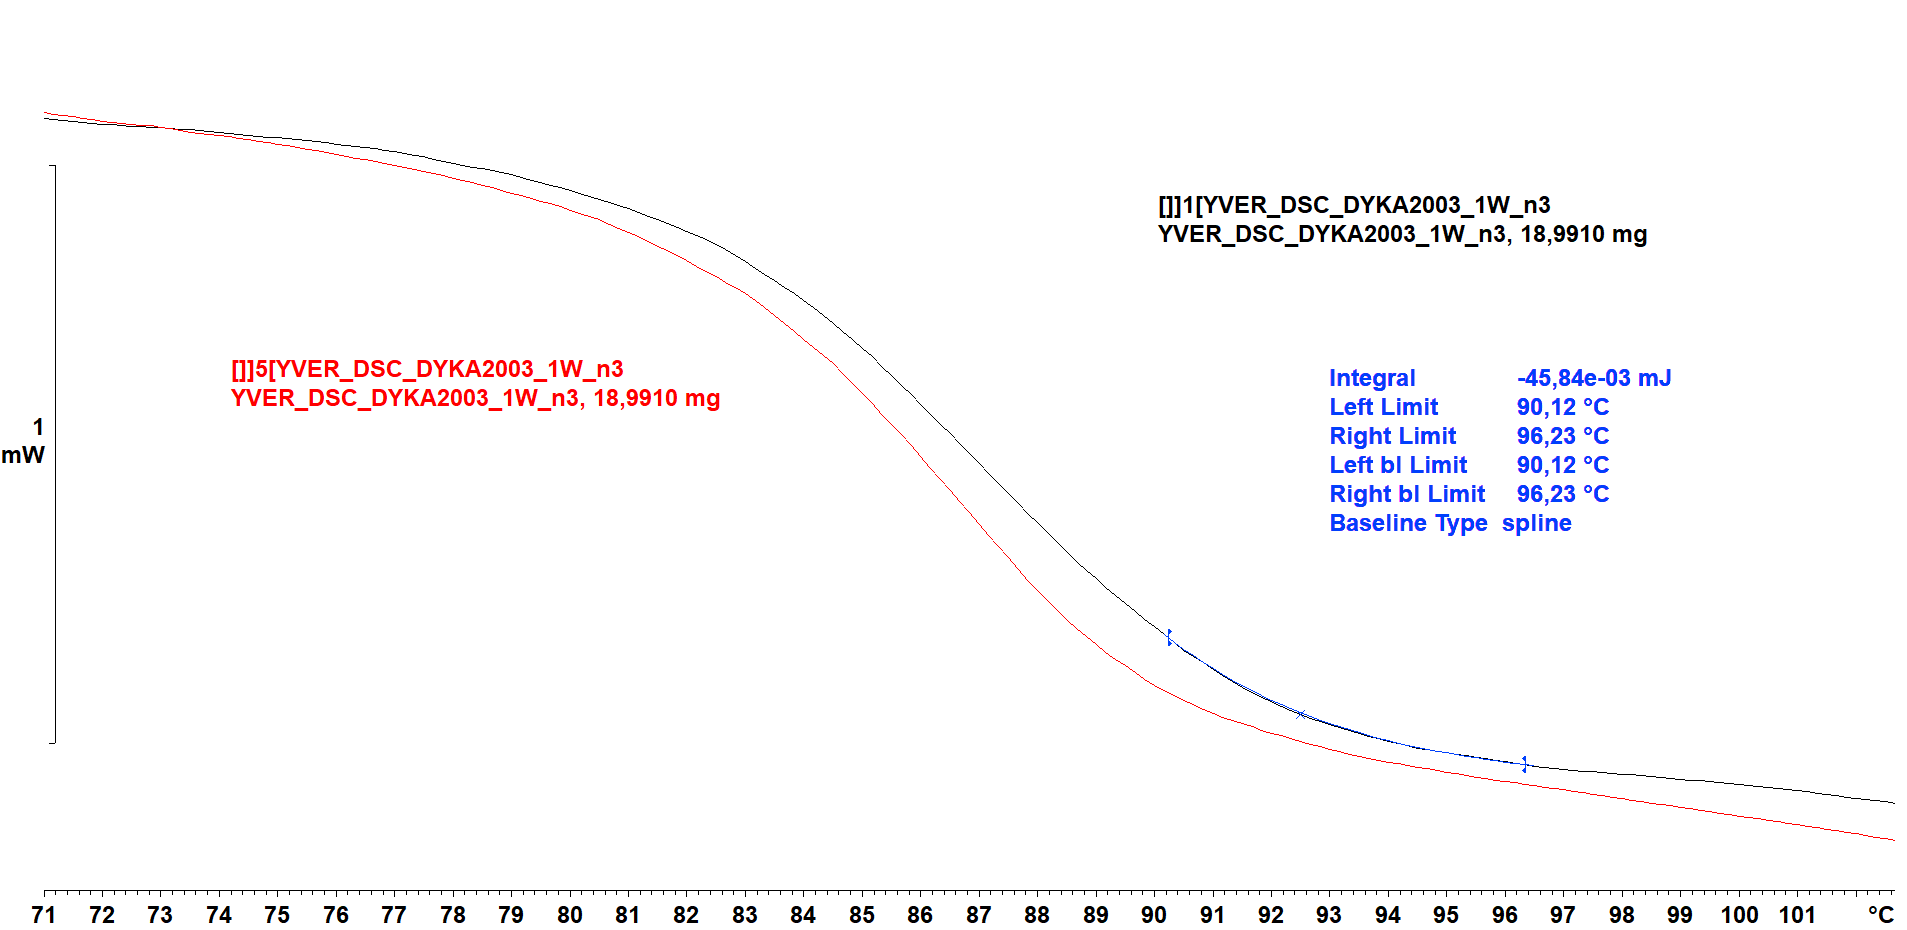
\includegraphics[width=0.75\linewidth]{DYKA2003_1w_n3.png}
    \caption{Endothermic peak of DYKA 2003, 1 week ageing, n°3}
    \label{fig:dyka2003_1w_n3}
\end{figure}
\begin{figure}[H]
    \centering
    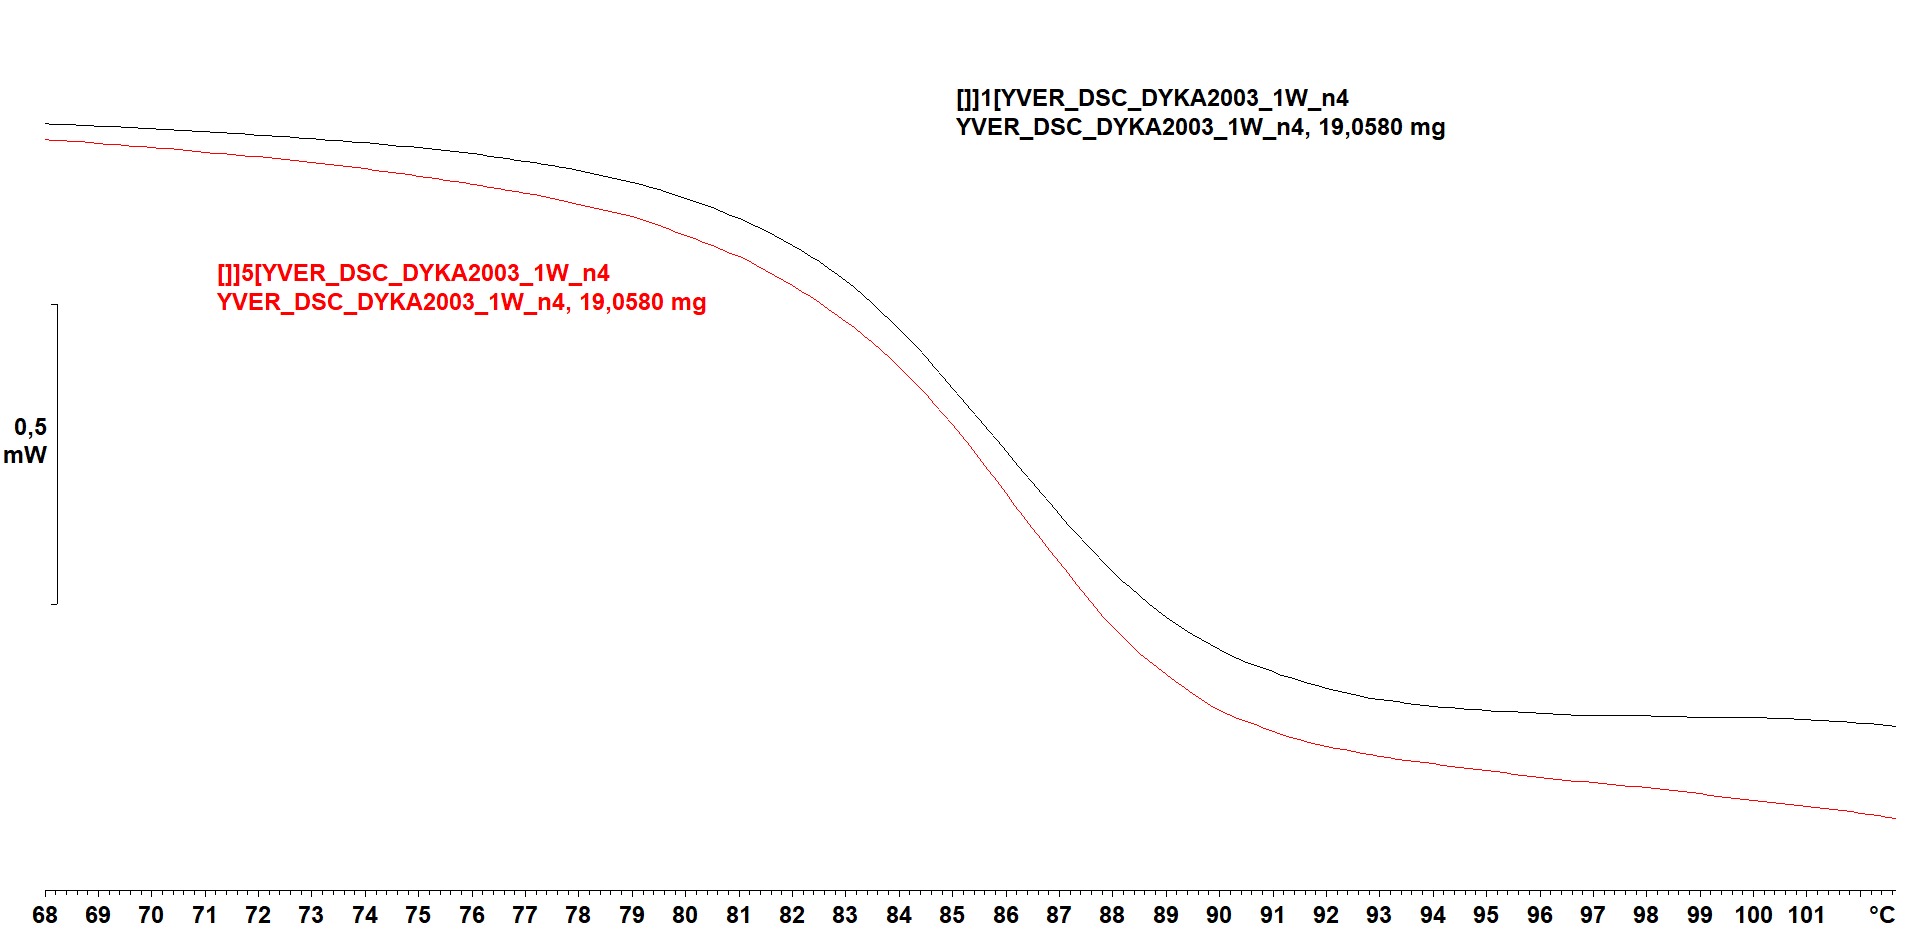
\includegraphics[width=0.75\linewidth]{DYKA2003_1w_n4.png}
    \caption{Endothermic peak of DYKA 2003, 1 week ageing, n°4}
    \label{fig:dyka2003_1w_n4}
\end{figure}

\subsubsection{2 weeks ageing}

\begin{figure}[H]
    \centering
    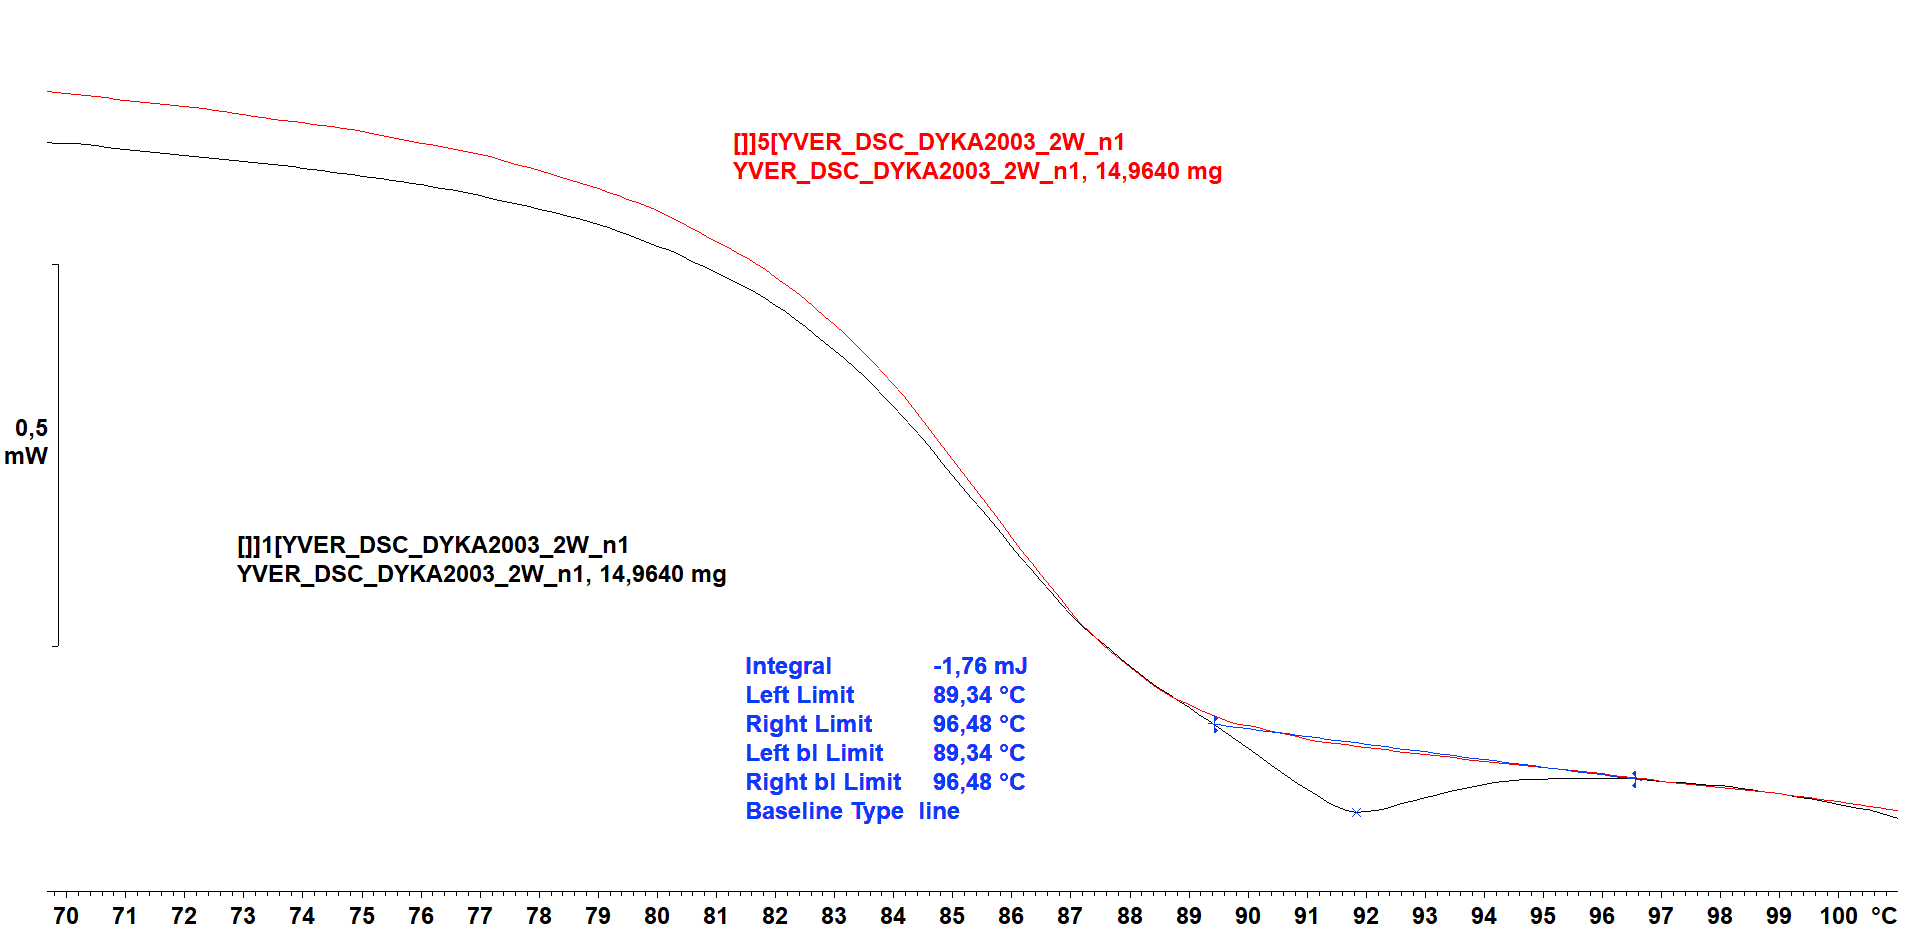
\includegraphics[width=0.75\linewidth]{DYKA2003_2w_n1.png}
    \caption{Endothermic peak of DYKA 2003, 2 weeks ageing, n°1}
    \label{fig:dyka2003_2w_n1}
\end{figure}

\begin{figure}[H]
    \centering
    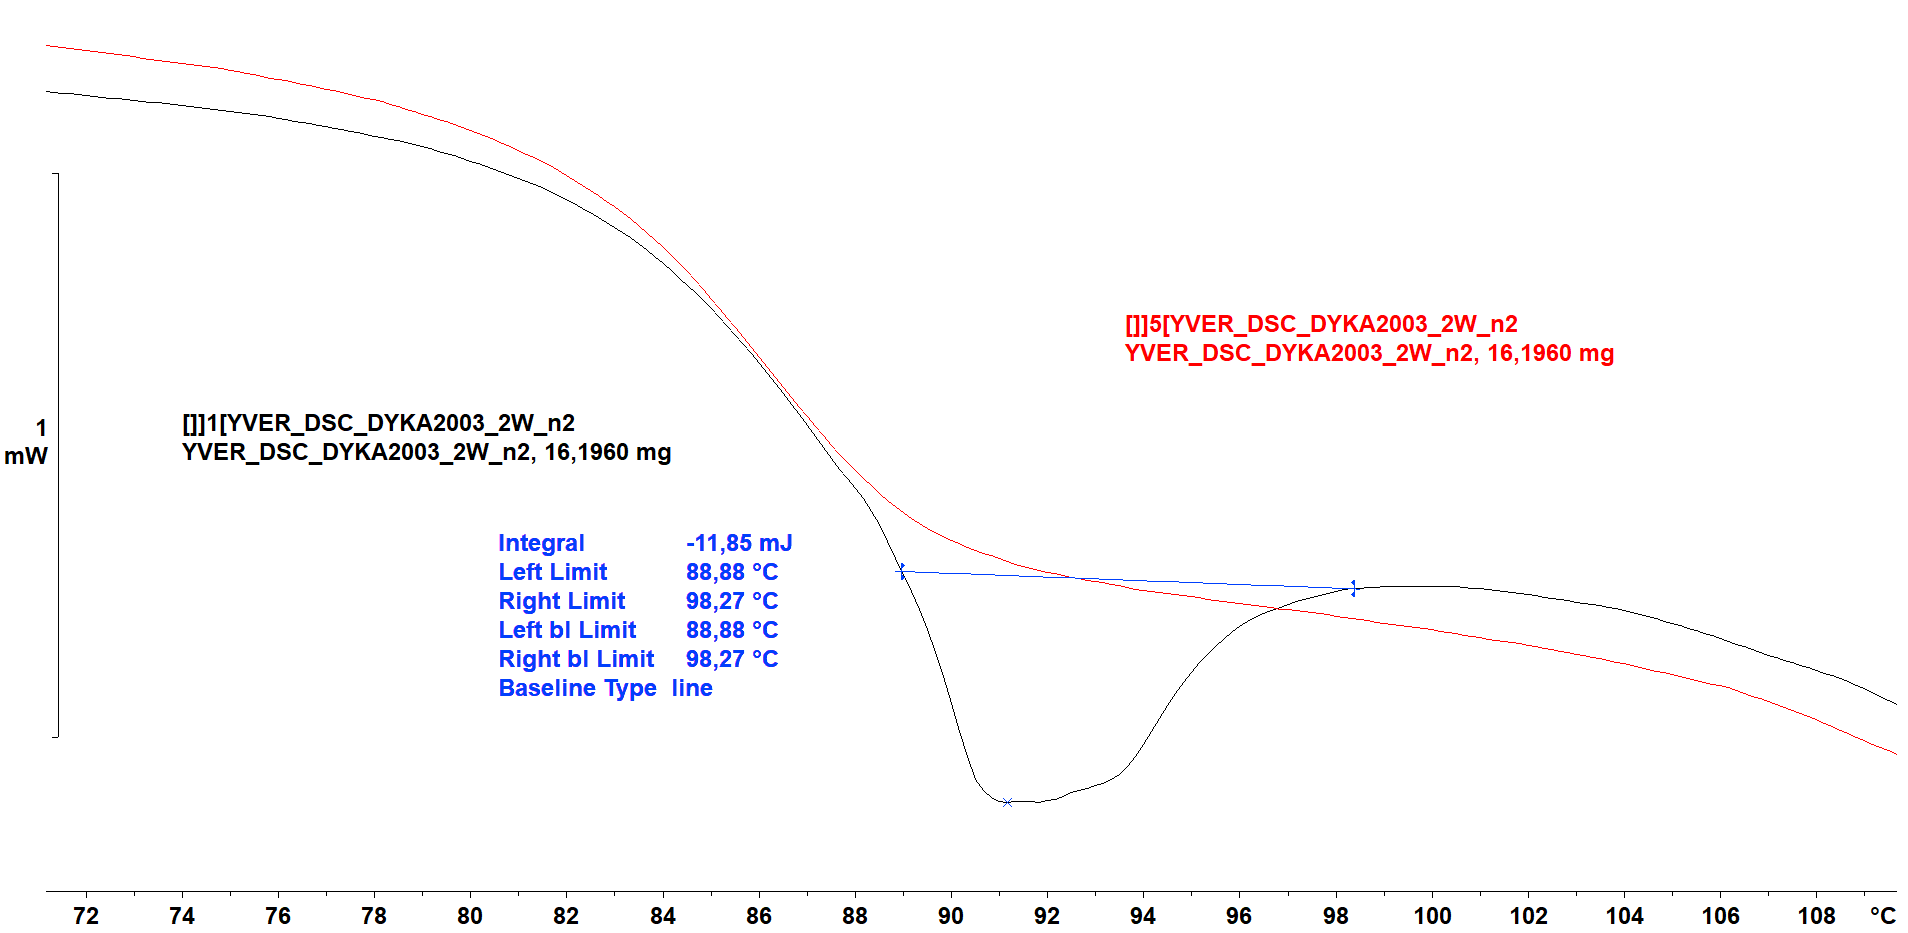
\includegraphics[width=0.75\linewidth]{DYKA2003_2w_n2.png}
    \caption{Endothermic peak of DYKA 2003, 2 weeks ageing, n°2}
    \label{fig:dyka2003_2w_n2}
\end{figure}

\begin{figure}[H]
    \centering
    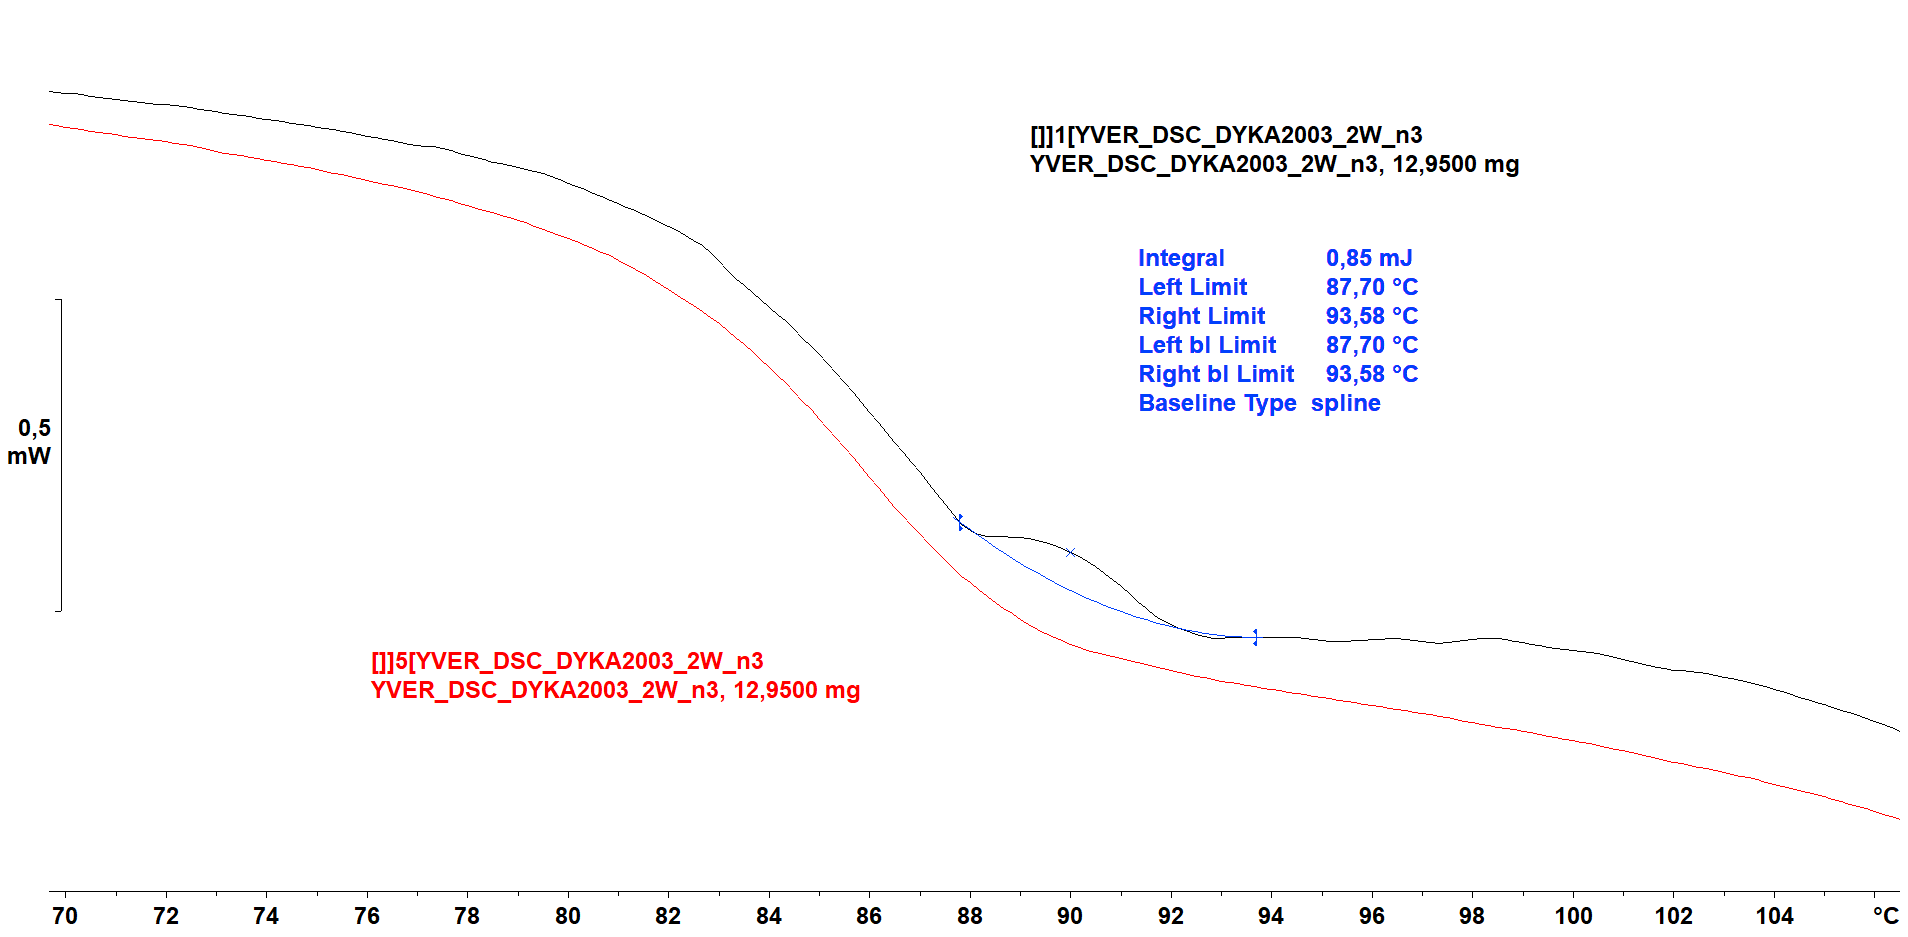
\includegraphics[width=0.75\linewidth]{DYKA2003_2w_n3.png}
    \caption{Endothermic peak of DYKA 2003, 2 weeks ageing, n°3}
    \label{fig:dyka2003_2w_n3}
\end{figure}

\begin{figure}[H]
    \centering
    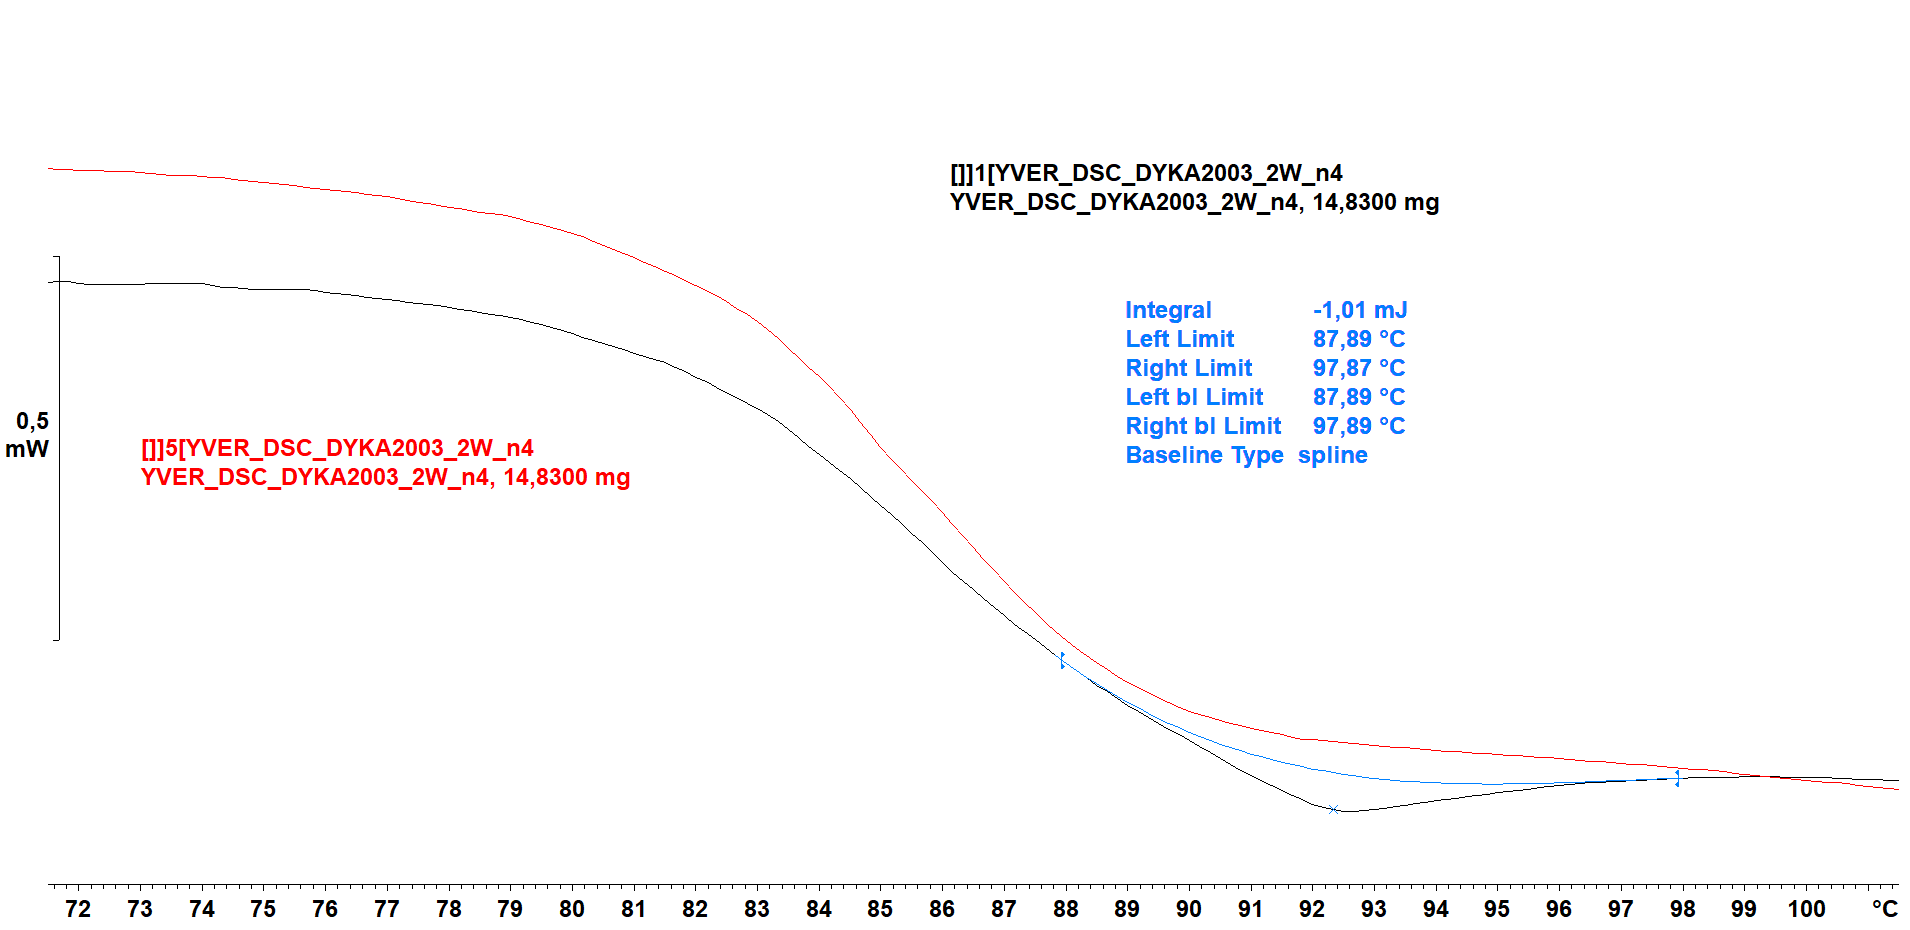
\includegraphics[width=0.75\linewidth]{DYKA2003_2w_n4.png}
    \caption{Endothermic peak of DYKA 2003, 2 weeks ageing, n°4}
    \label{fig:dyka2003_2w_n4}
\end{figure}

\subsection{Wavin 1987}
\subsubsection{0 day ageing}
\begin{figure}[H]
    \centering
    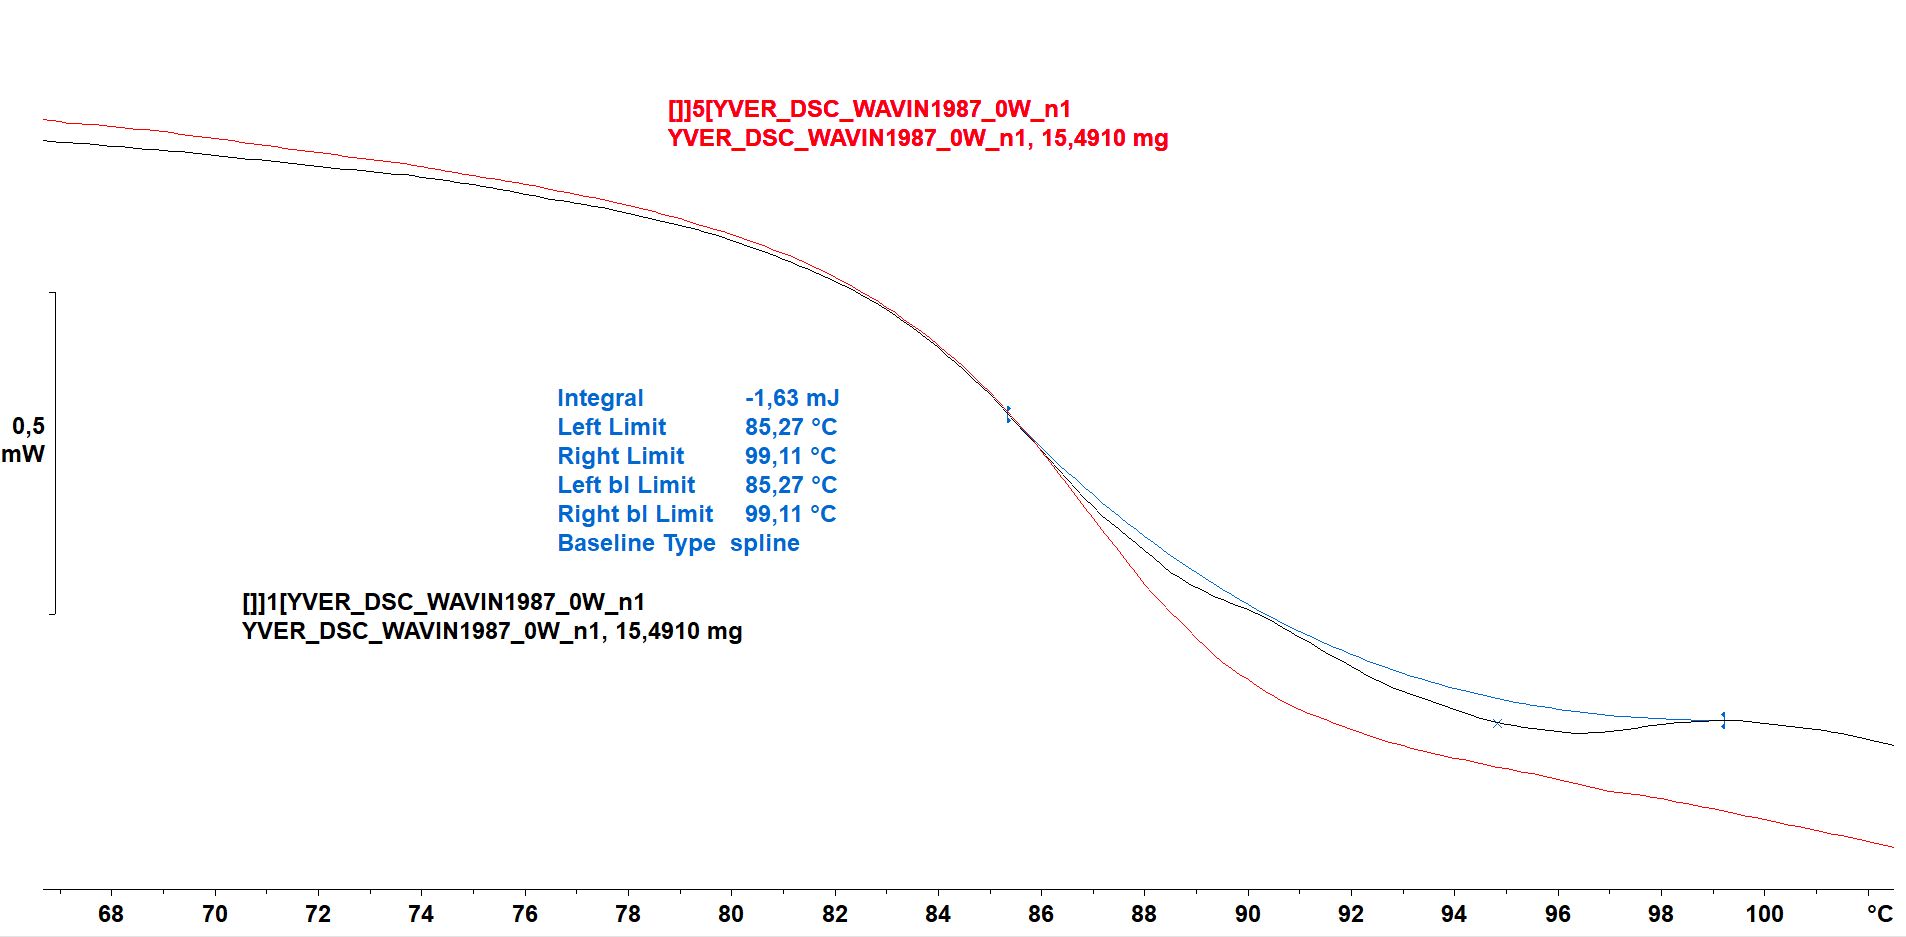
\includegraphics[width=0.75\linewidth]{wavin1987_DSC_0d_n1.png}
    \caption{Endothermic peak of Wavin 1987, 0 day ageing, n°1}
    \label{fig:wavin1987_0d_n1}
\end{figure}

\begin{figure}[H]
    \centering
    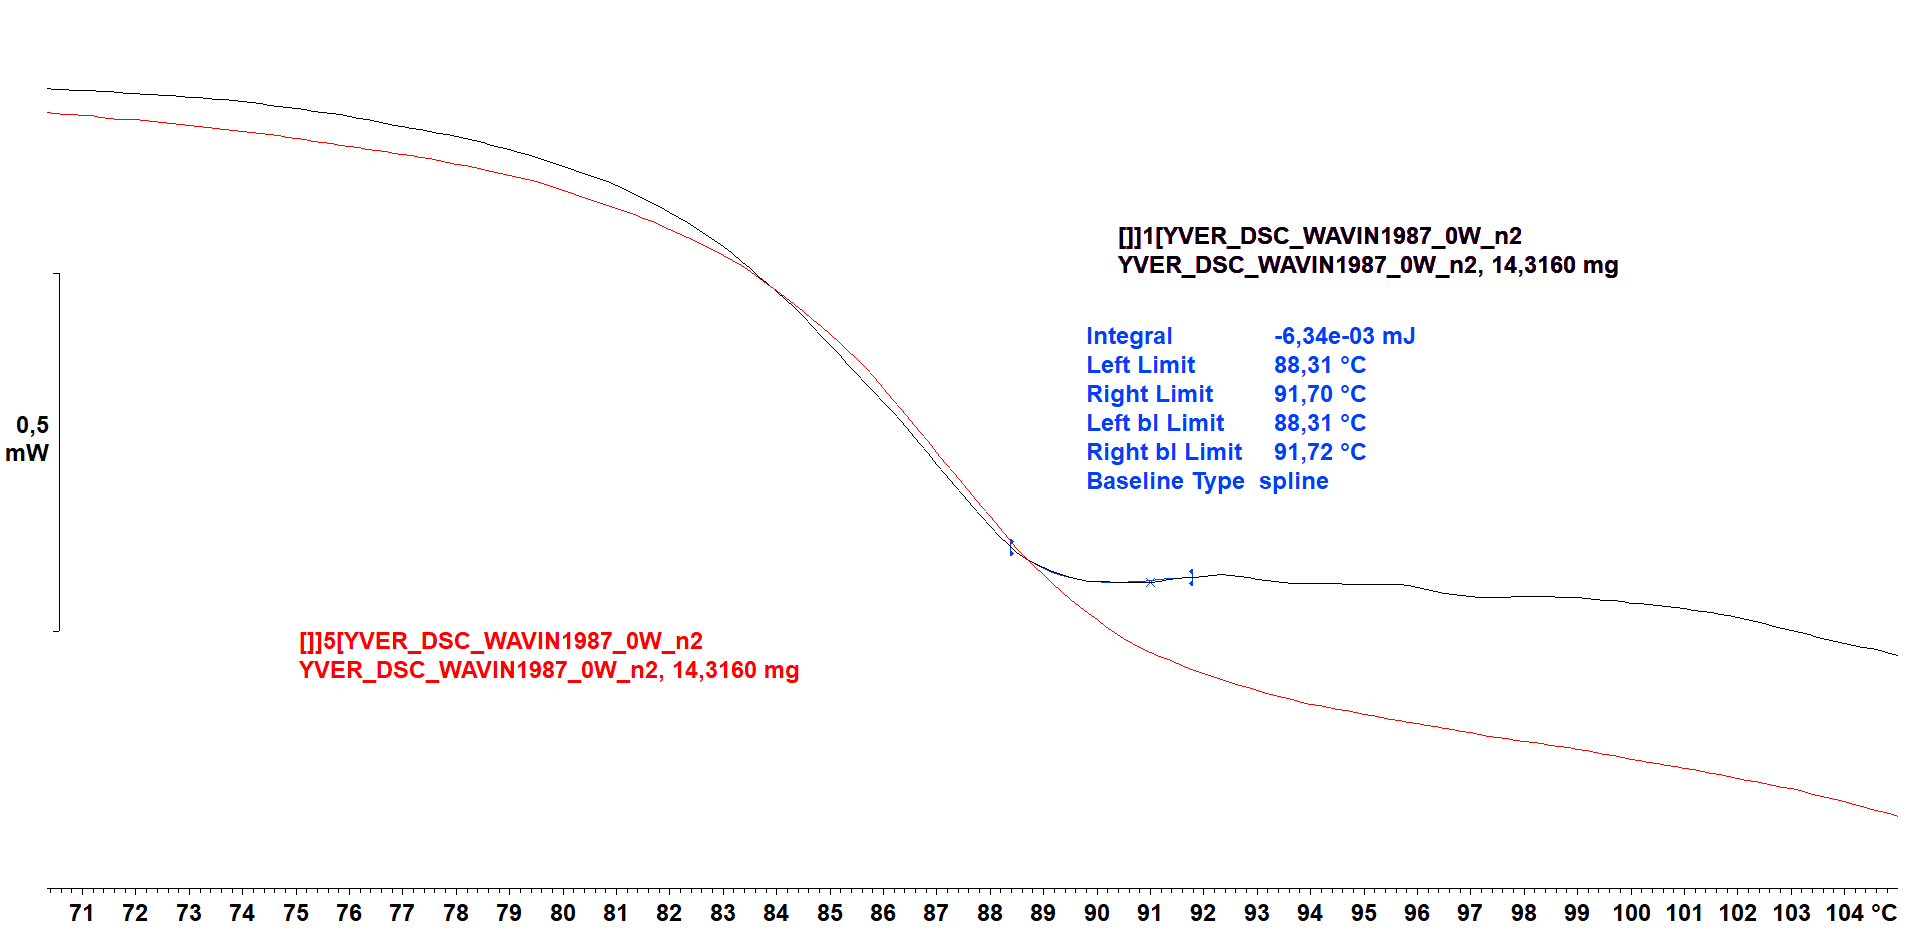
\includegraphics[width=0.75\linewidth]{Wavin1987_DSC_0d_n2.png}
    \caption{Endothermic peak of Wavin 1987, 0 day ageing, n°2}
    \label{fig:wavin1987_0d_n2}
\end{figure}

\begin{figure}[H]
    \centering
    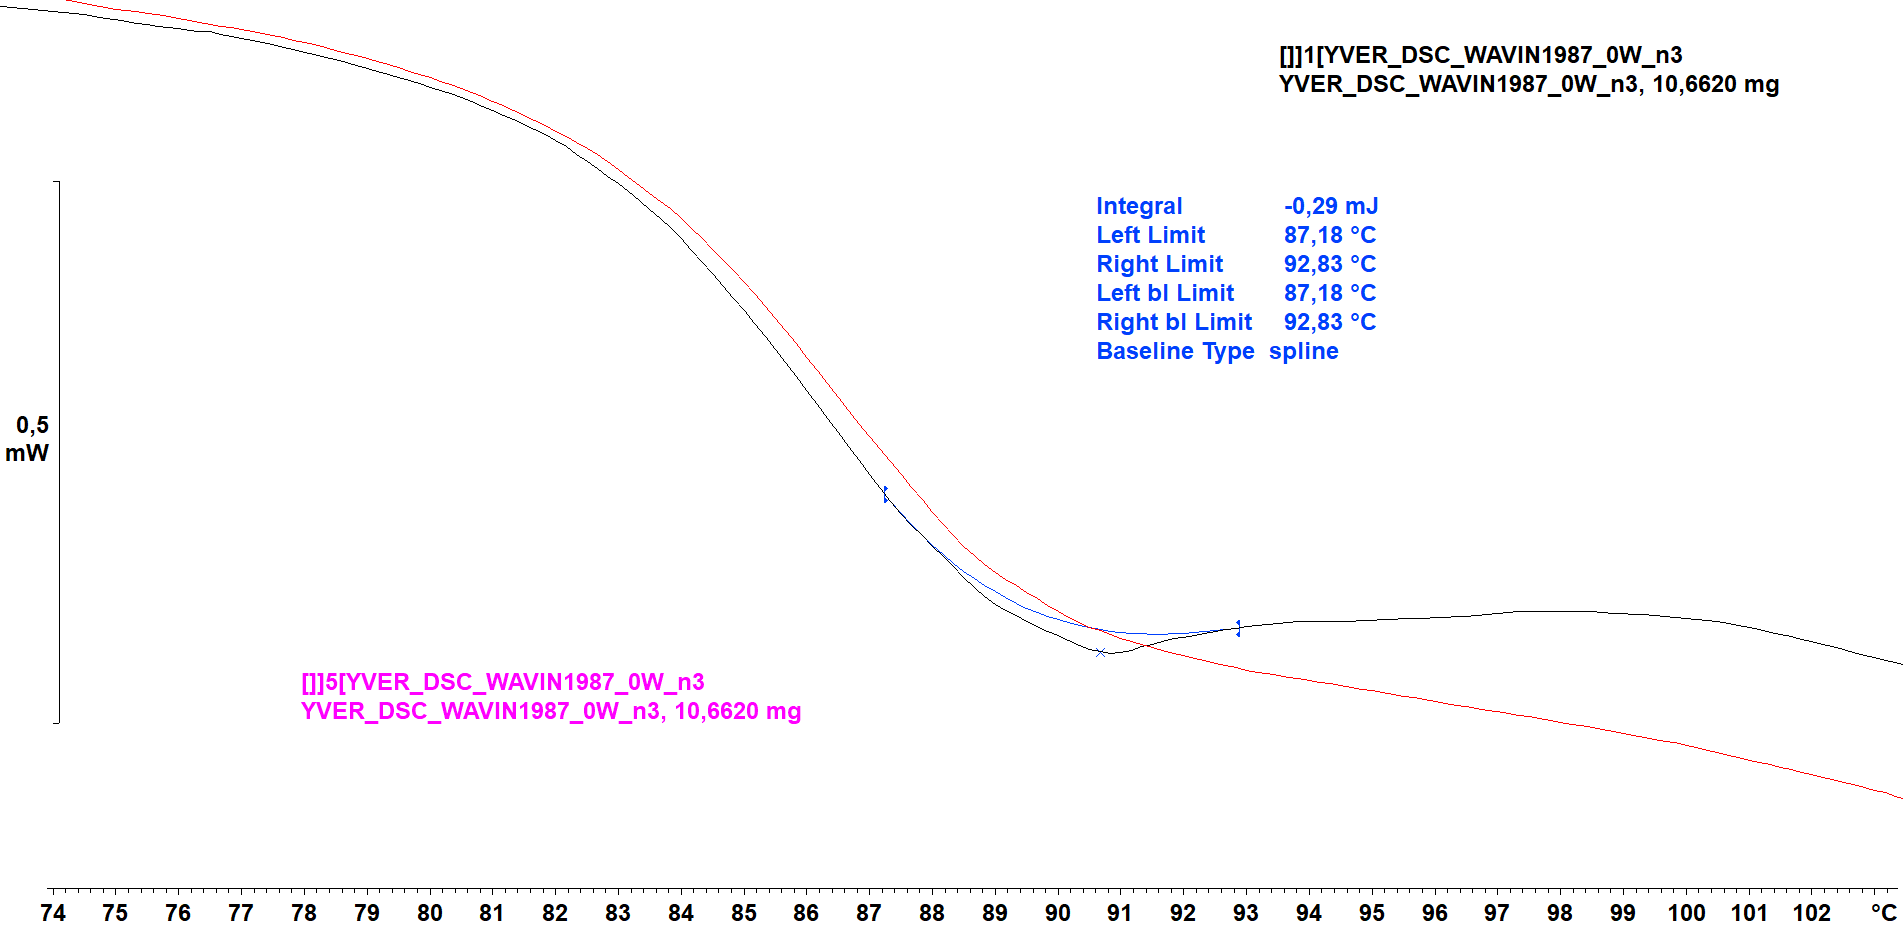
\includegraphics[width=0.75\linewidth]{Wavin1987_DSC_0d_n3.png}
    \caption{Endothermic peak of Wavin 1987, 0 day ageing, n°3}
    \label{fig:wavin1987_0d_n3}
\end{figure}

\begin{figure}[H]
    \centering
    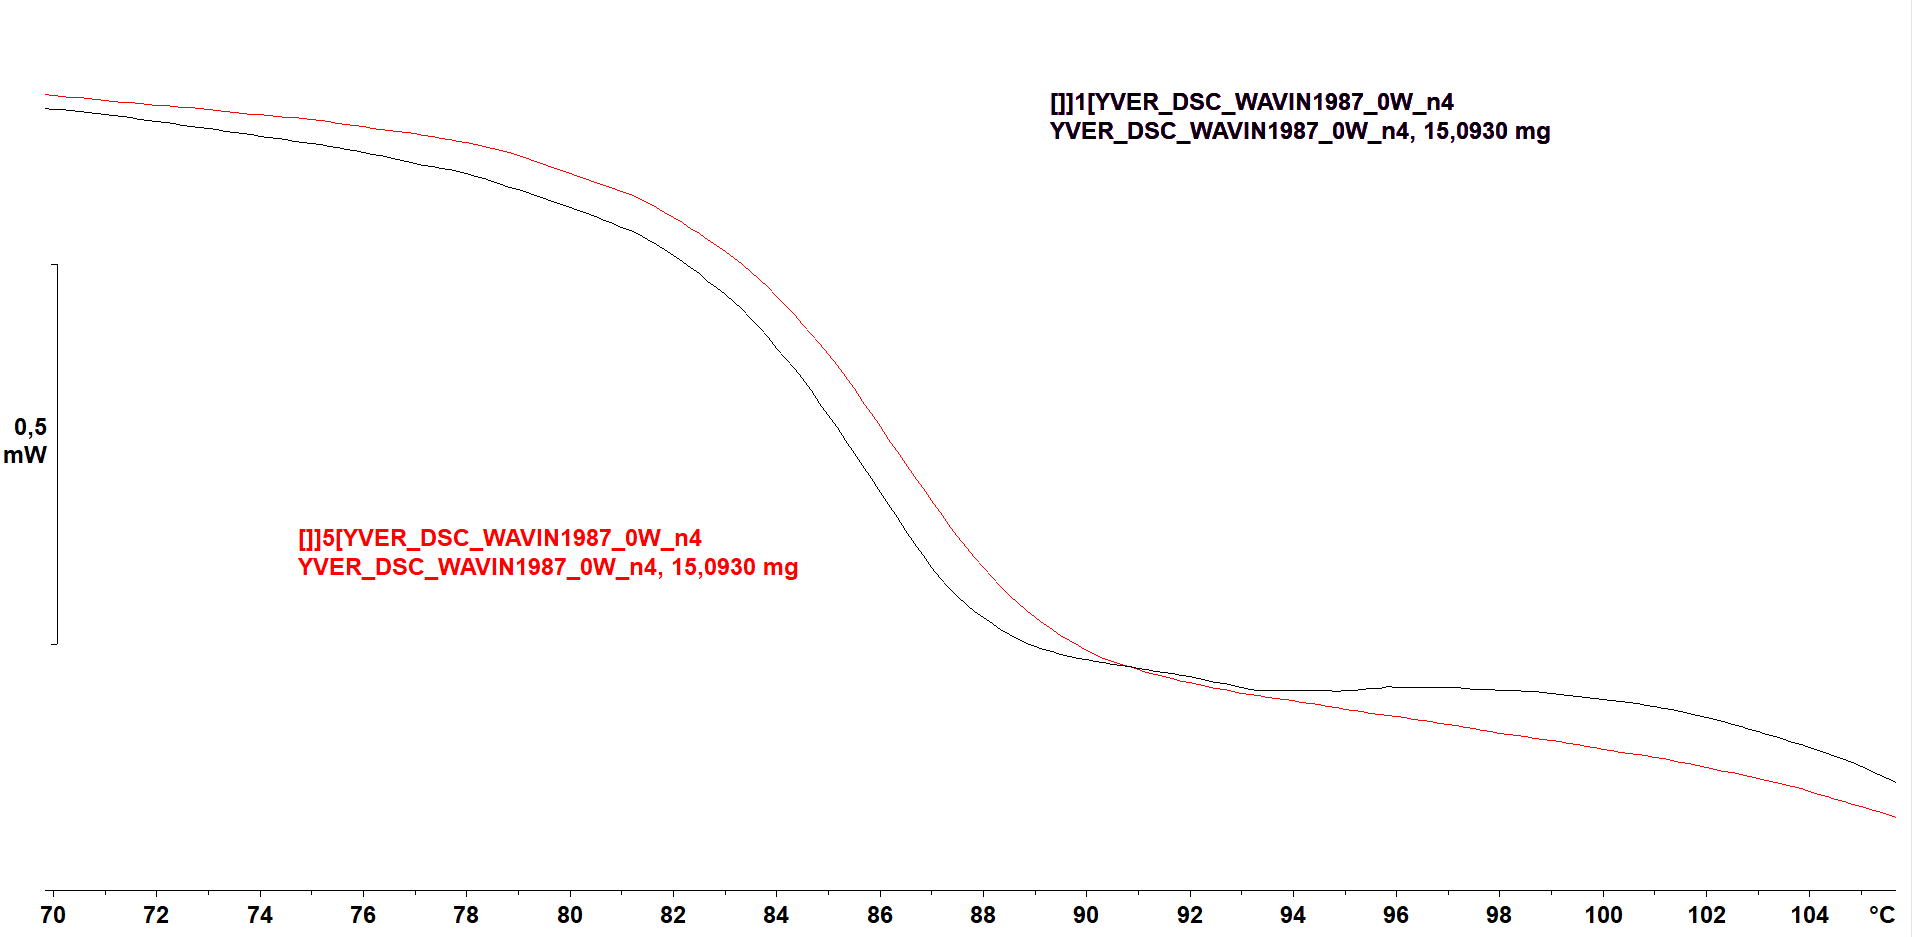
\includegraphics[width=0.75\linewidth]{Wavin1987_DSC_0d_n4.png}
    \caption{Endothermic peak of Wavin 1987, 0 day ageing, n°4}
    \label{fig:wavin1987_0d_n4}
\end{figure}
\subsubsection{4 days ageing}
\begin{figure}[H]
    \centering
    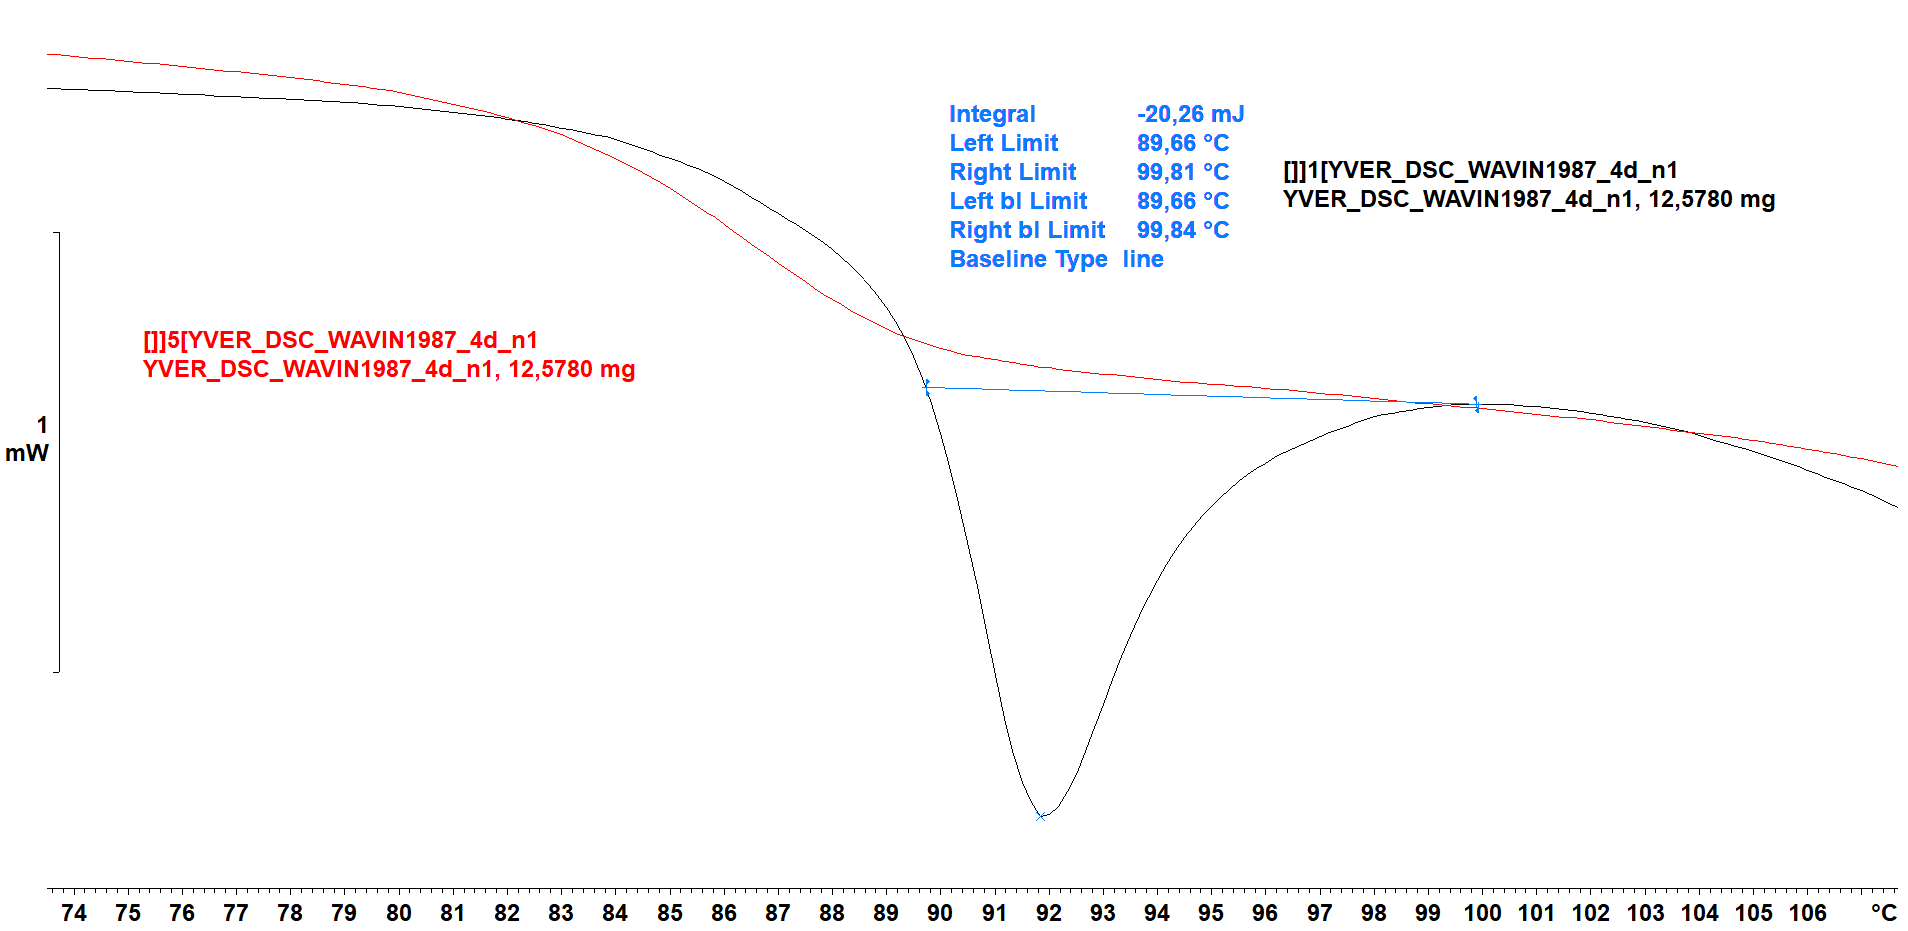
\includegraphics[width=0.75\linewidth]{Wavin1987_DSC_4d_n1.png}
    \caption{Endothermic peak of Wavin 1987, 4 days ageing, n°1}
    \label{fig:wavin1987_4d_n1}
\end{figure}
\begin{figure}[H]
    \centering
    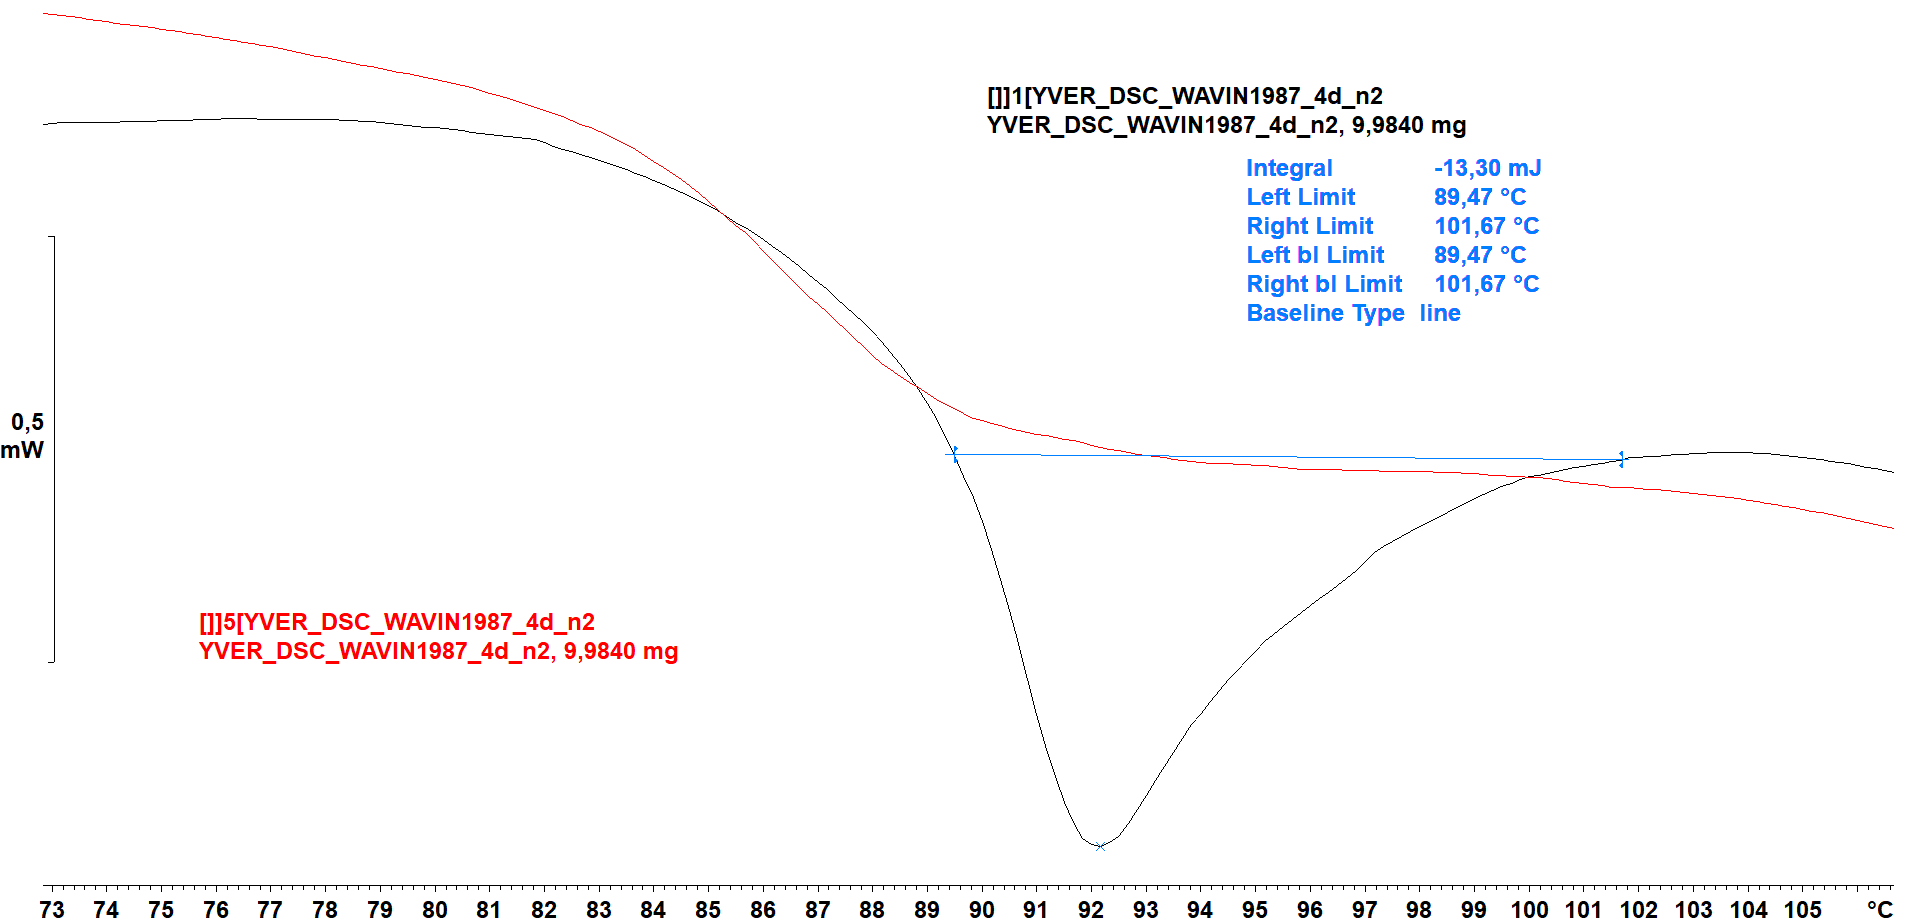
\includegraphics[width=0.75\linewidth]{Wavin1987_DSC_4d_n2.png}
    \caption{Endothermic peak of Wavin 1987, 4 days ageing, n°2}
    \label{fig:wavin1987_4d_n2}
\end{figure}
\begin{figure}[H]
    \centering
    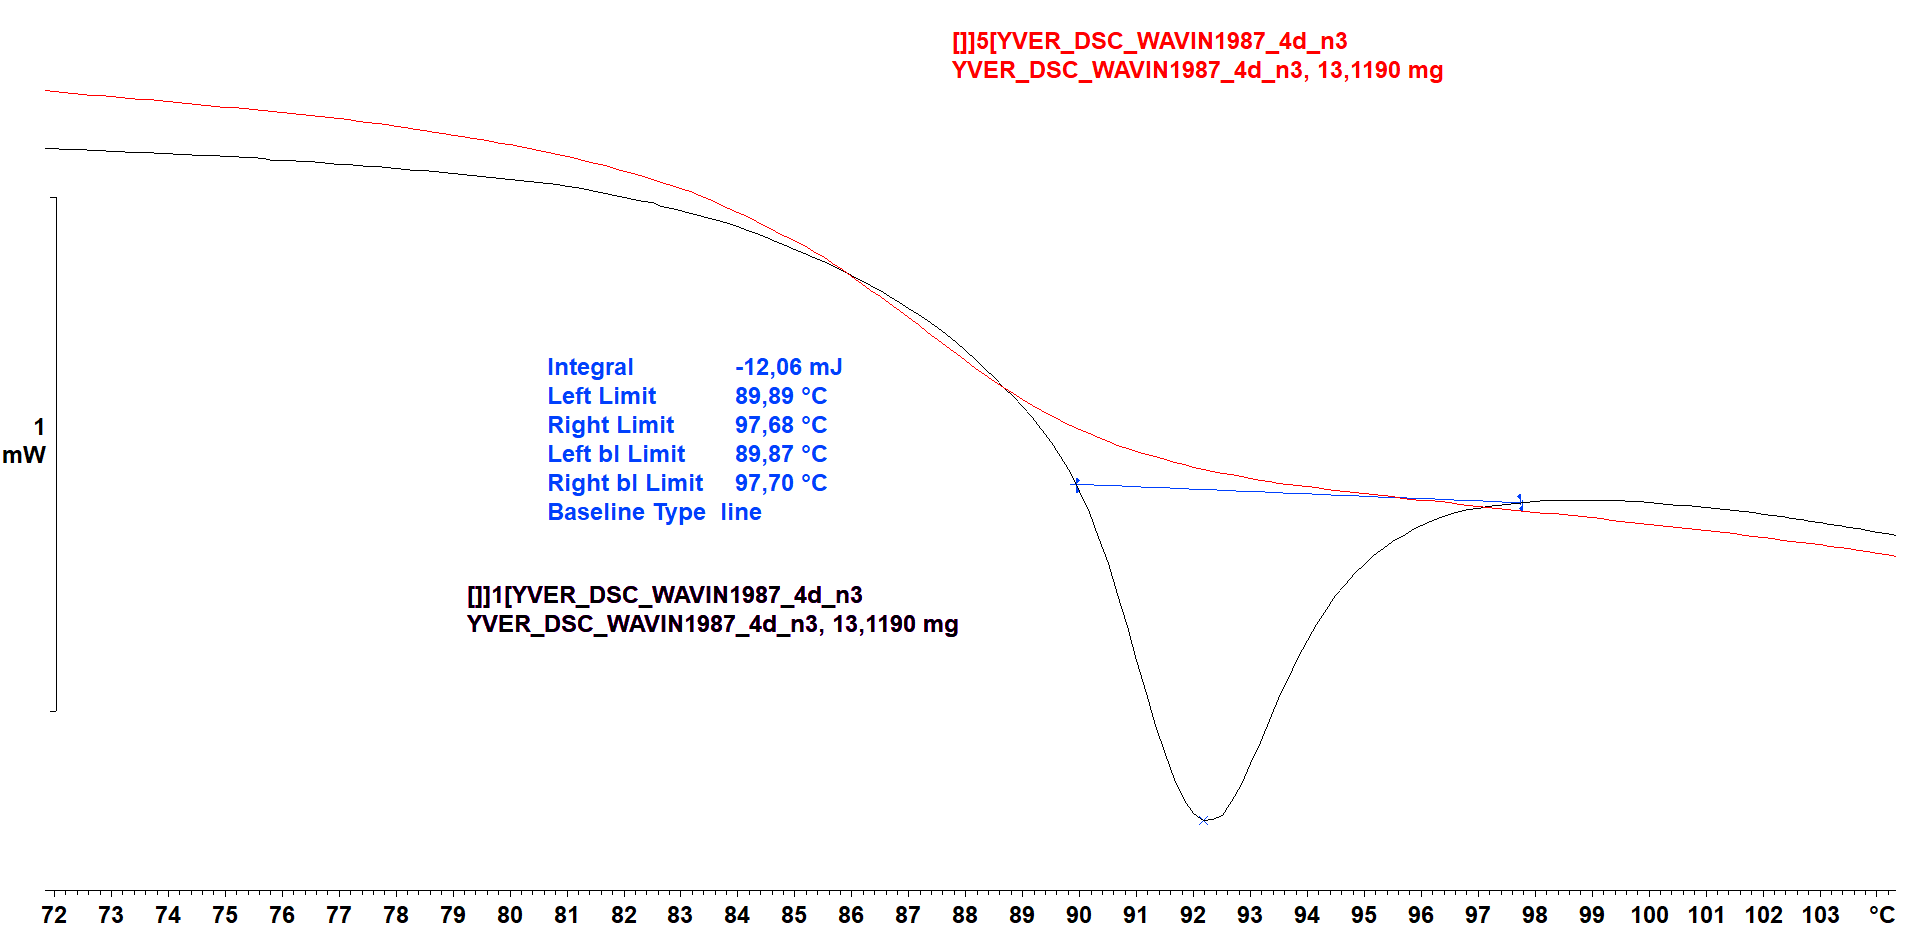
\includegraphics[width=0.75\linewidth]{Wavin1987_DSC_4d_n3.png}
    \caption{Endothermic peak of Wavin 1987, 4 days ageing, n°3}
    \label{fig:wavin1987_4d_n3}
\end{figure}
\begin{figure}[H]
    \centering
    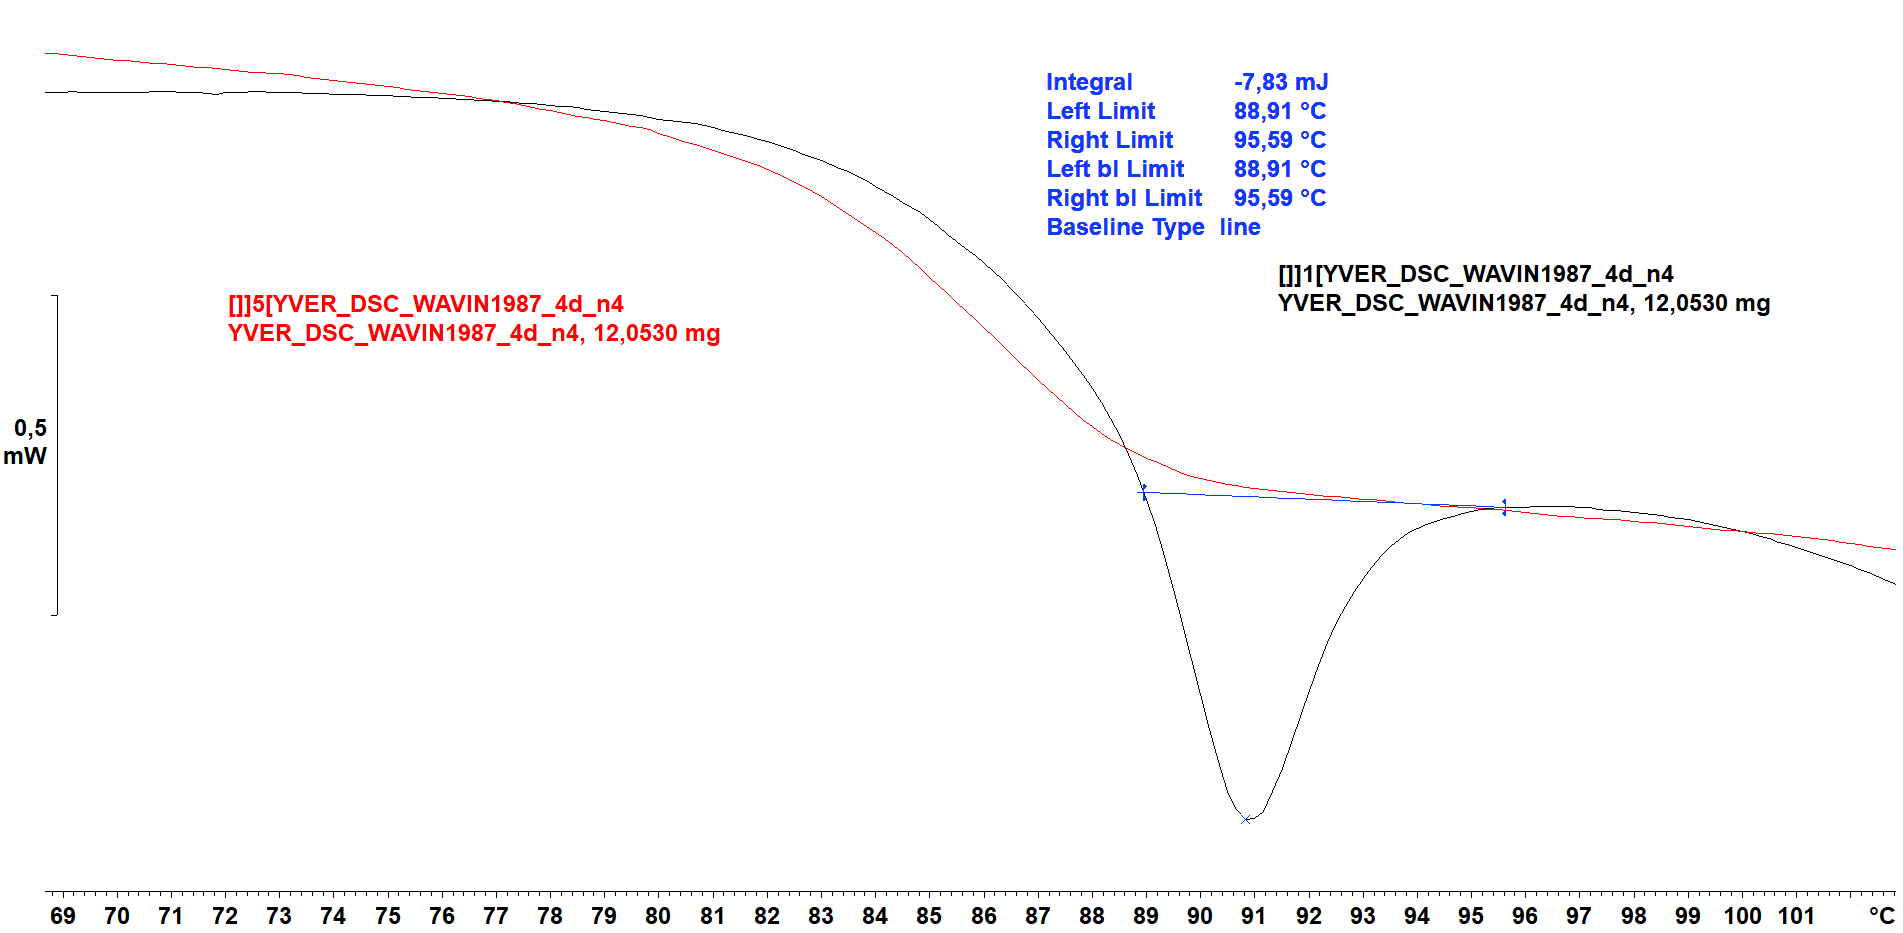
\includegraphics[width=0.75\linewidth]{Wavin1987_DSC_4d_n4.png}
    \caption{Endothermic peak of Wavin 1987, 4 days ageing, n°4}
    \label{fig:wavin1987_4d_n4}
\end{figure}
\subsubsection{1 week ageing}
\begin{figure}[H]
    \centering
    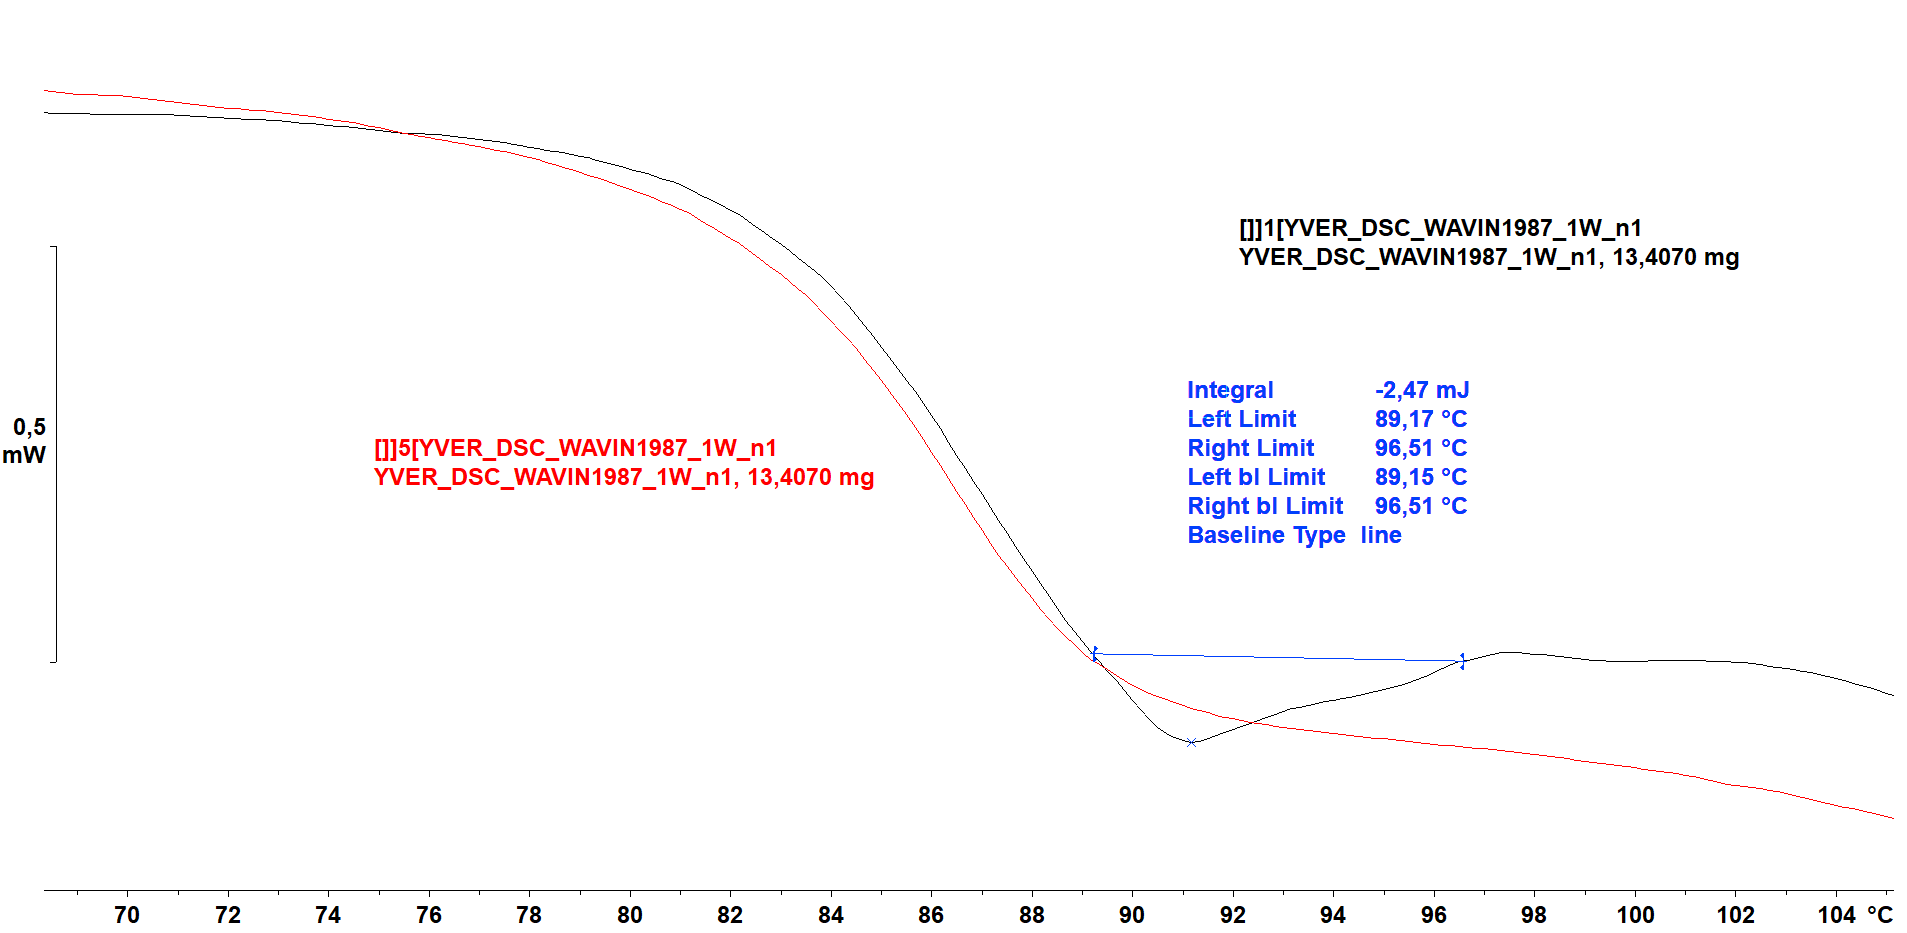
\includegraphics[width=0.75\linewidth]{Wavin1987_DSC_1w_n1.png}
    \caption{Endothermic peak of Wavin 1987, 1 week ageing, n°1}
    \label{fig:wavin1987_1w_n1}
\end{figure}
\begin{figure}[H]
    \centering
    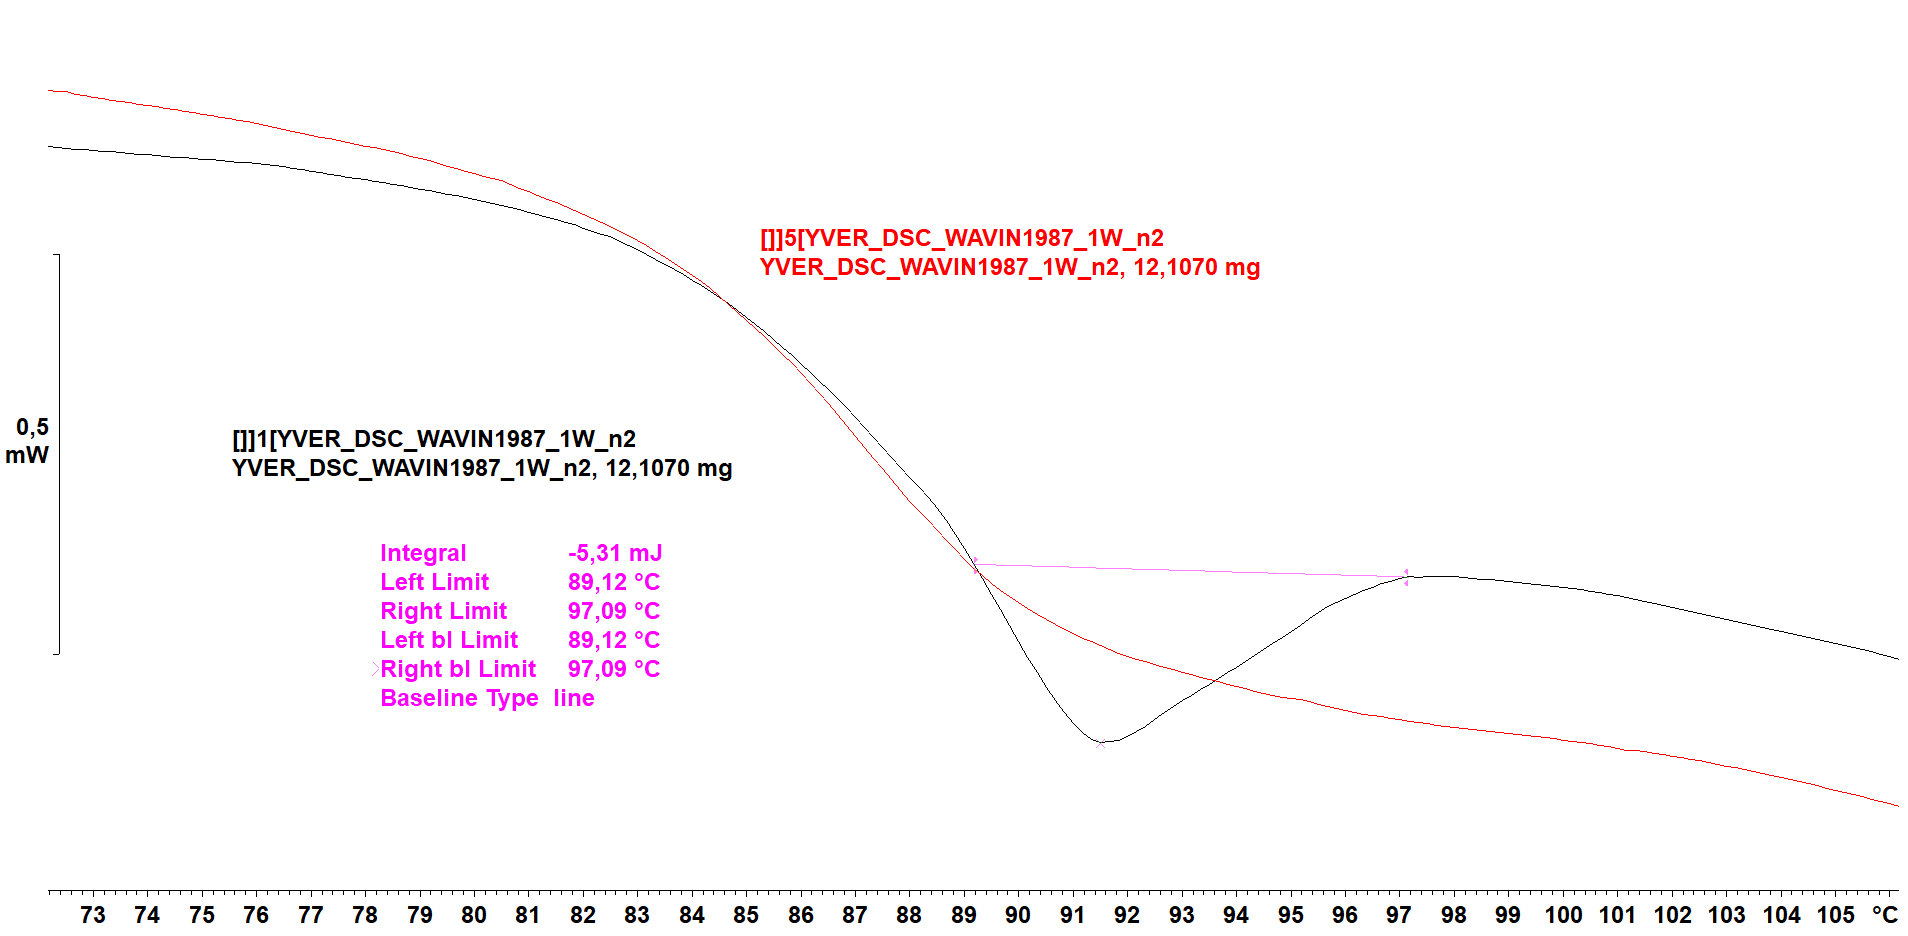
\includegraphics[width=0.75\linewidth]{Wavin1987_DSC_1w_n2.png}
    \caption{Endothermic peak of Wavin 1987, 1 week ageing, n°2}
    \label{fig:wavin1987_1w_n2}
\end{figure}
\begin{figure}[H]
    \centering
    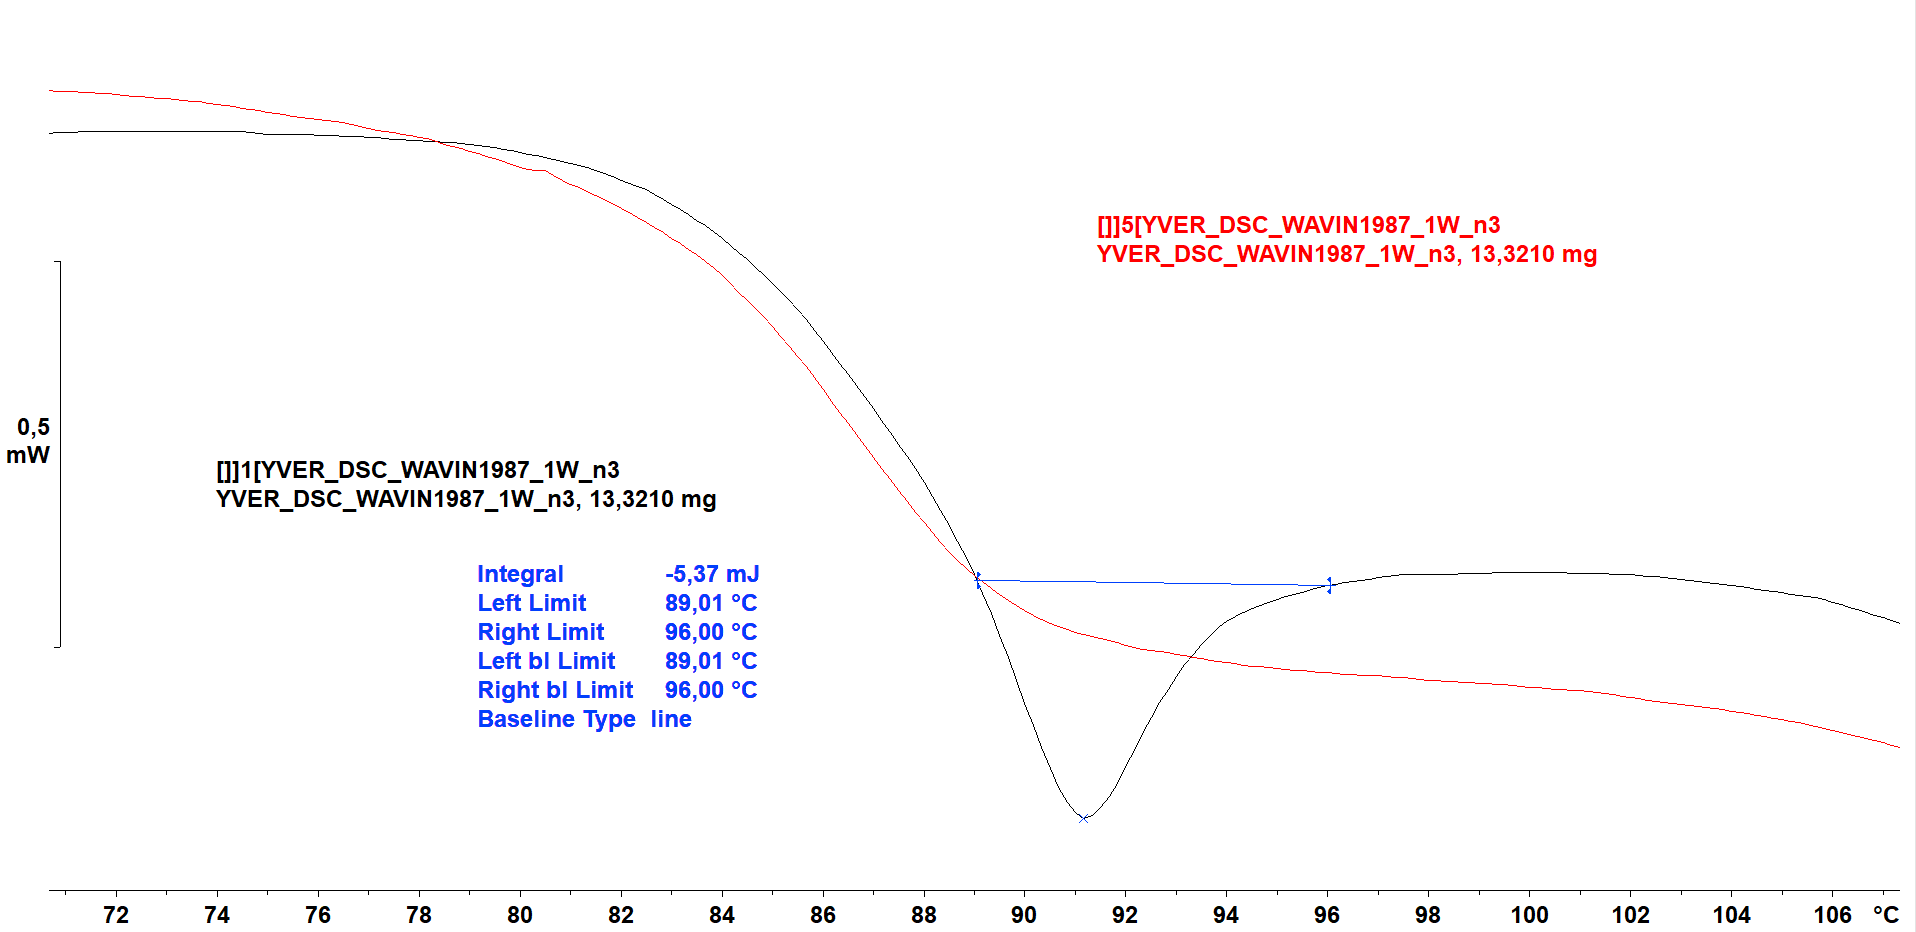
\includegraphics[width=0.75\linewidth]{Wavin1987_DSC_1w_n3.png}
    \caption{Endothermic peak of Wavin 1987, 1 week ageing, n°3}
    \label{fig:wavin1987_1w_n3}
\end{figure}
\begin{figure}[H]
    \centering
    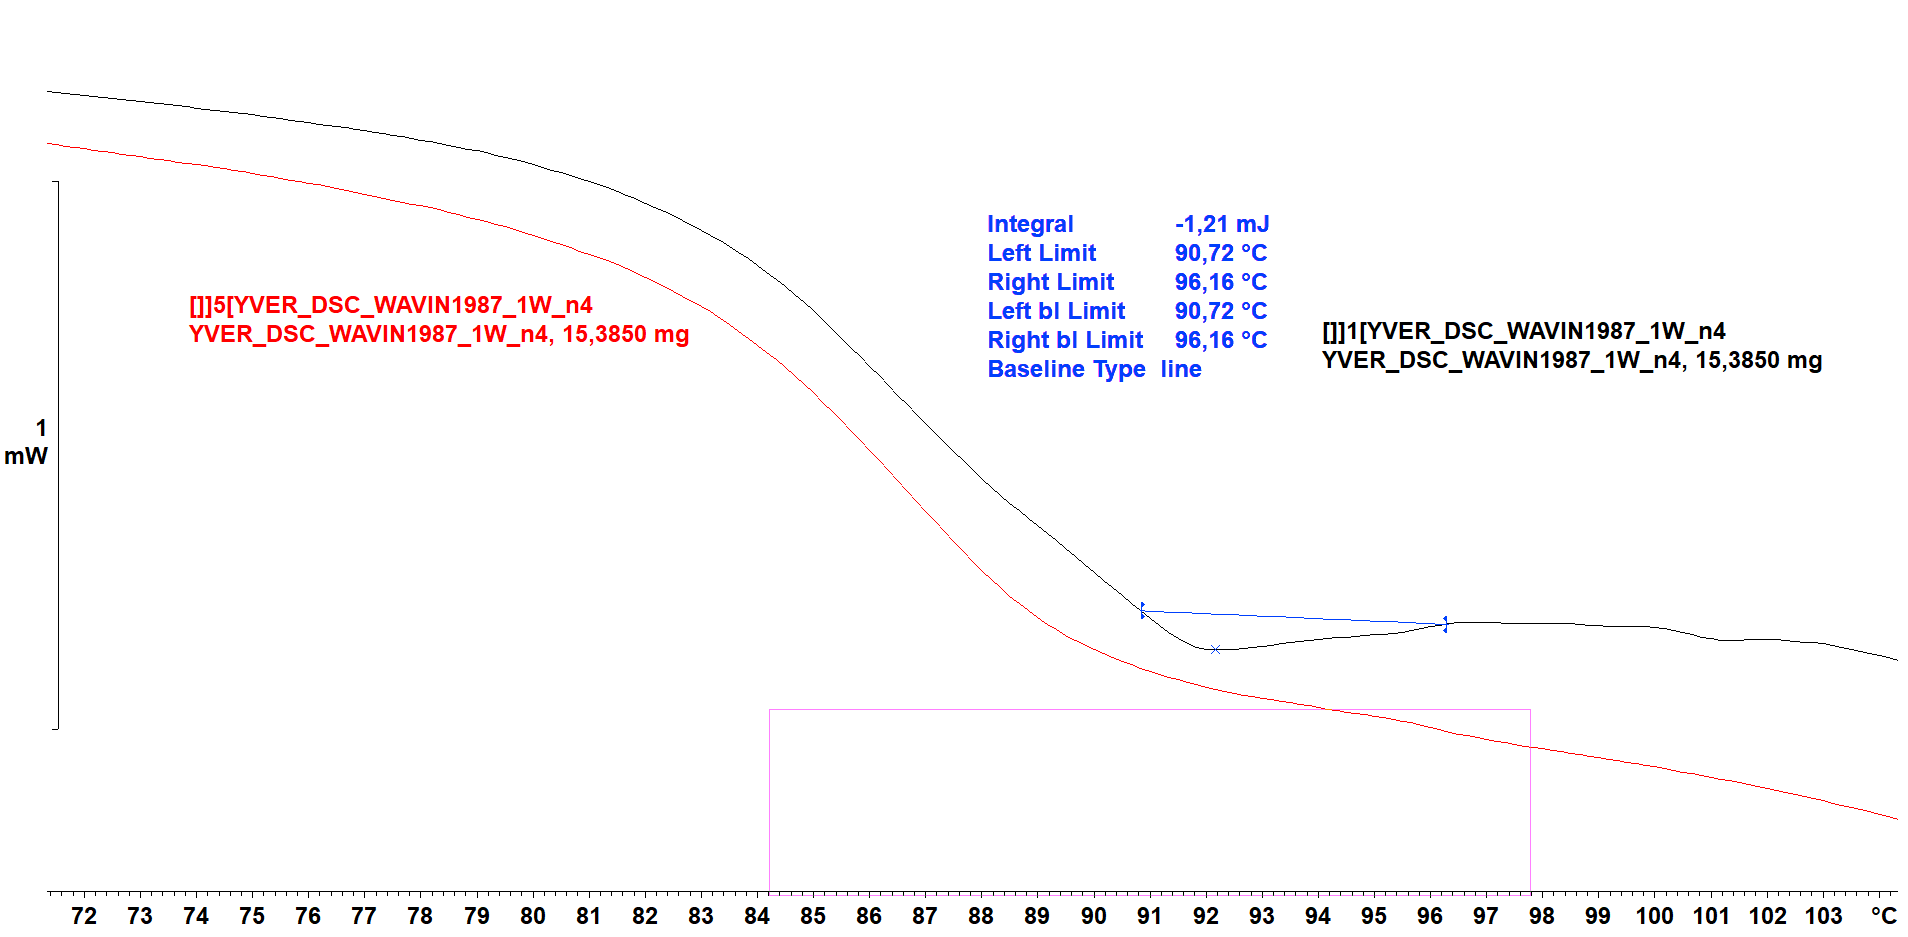
\includegraphics[width=0.75\linewidth]{Wavin1987_DSC_1w_n4.png}
    \caption{Endothermic peak of Wavin 1987, 1 week ageing, n°4}
    \label{fig:wavin1987_1w_n4}
\end{figure}
\subsubsection{2 weeks ageing}
\begin{figure}[H]
    \centering
    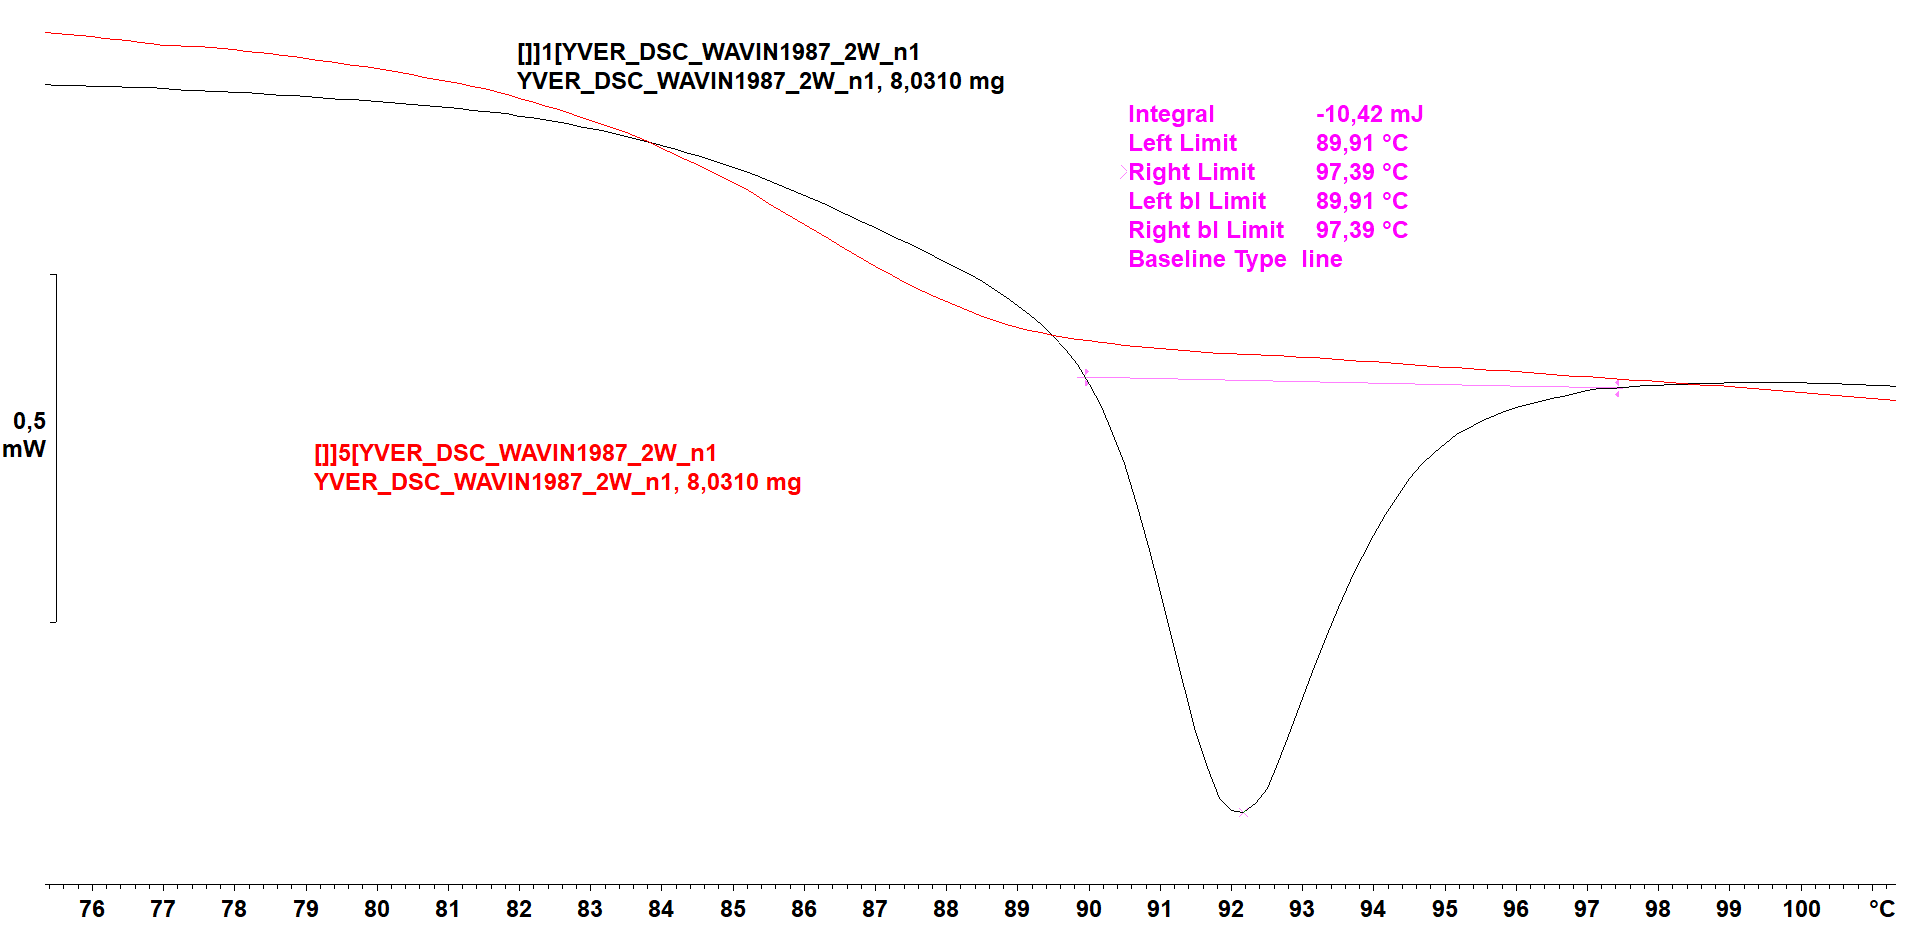
\includegraphics[width=0.75\linewidth]{Wavin1987_DSC_2w_n1.png}
    \caption{Endothermic peak of Wavin 1987, 2 weeks ageing, n°1}
    \label{fig:wavin1987_2w_n1}
\end{figure}
\begin{figure}[H]
    \centering
    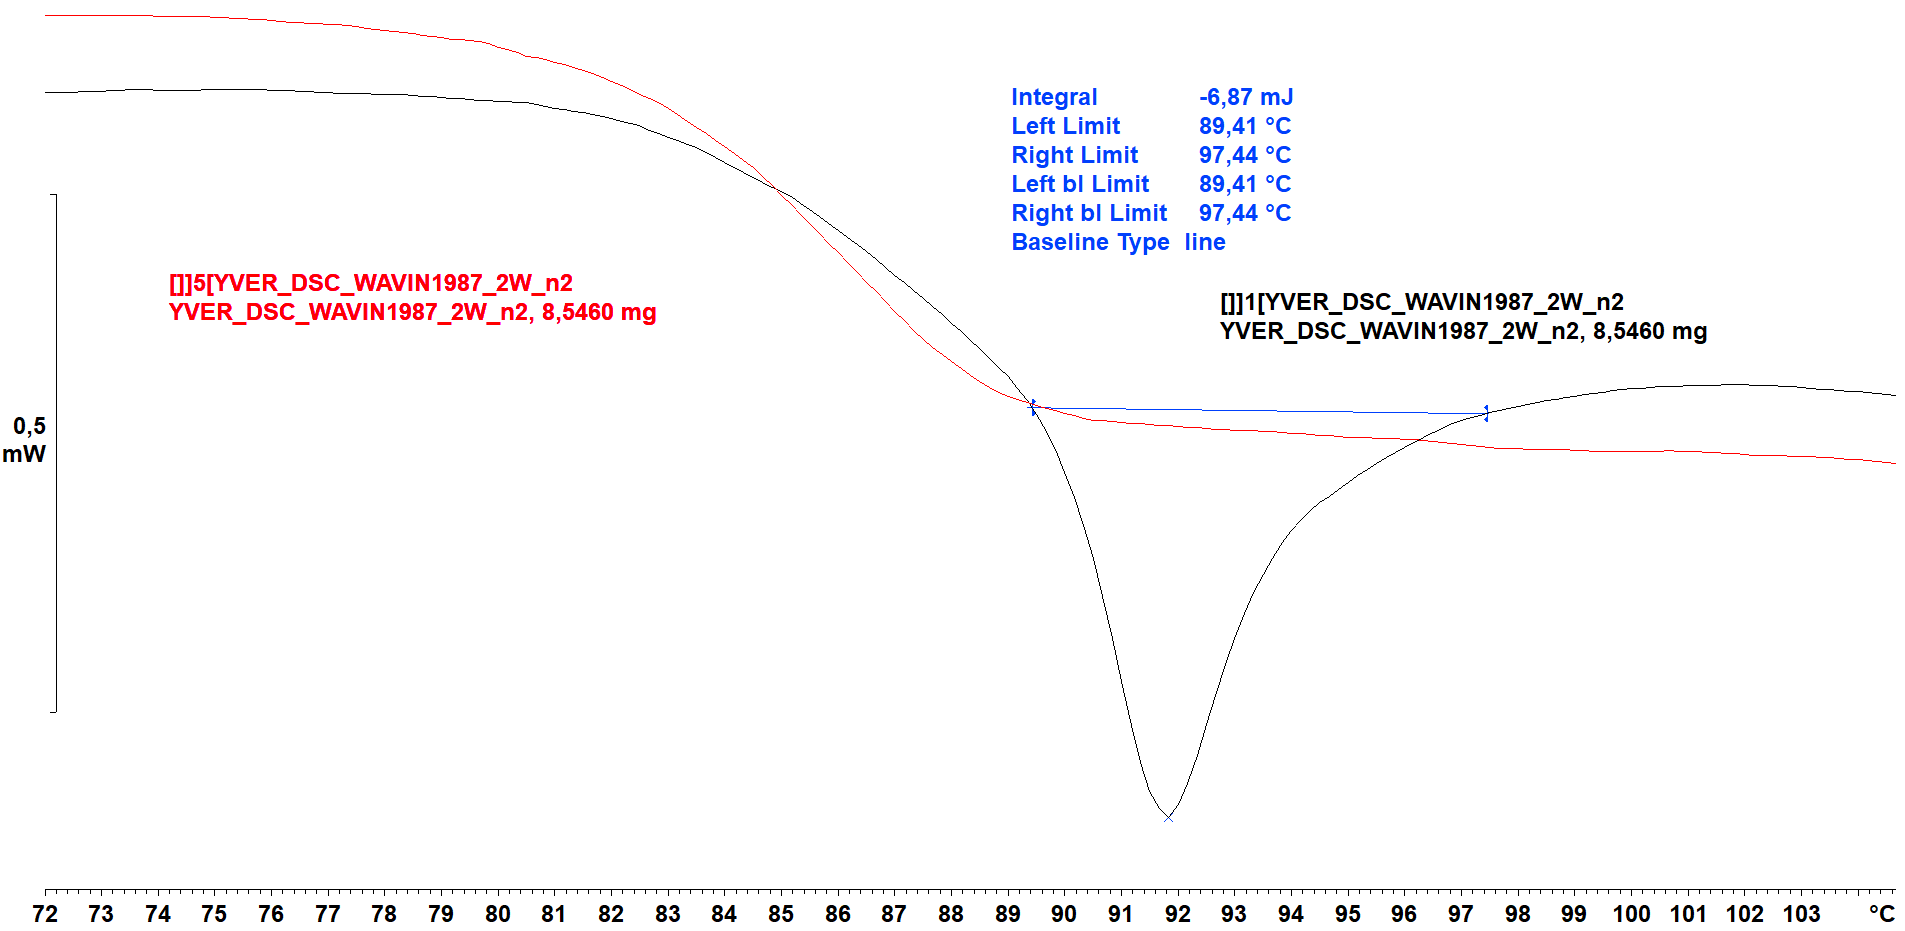
\includegraphics[width=0.75\linewidth]{Wavin1987_DSC_2w_n2.png}
    \caption{Endothermic peak of Wavin 1987, 2 weeks ageing, n°2}
    \label{fig:wavin1987_2w_n2}
\end{figure}
\begin{figure}[H]
    \centering
    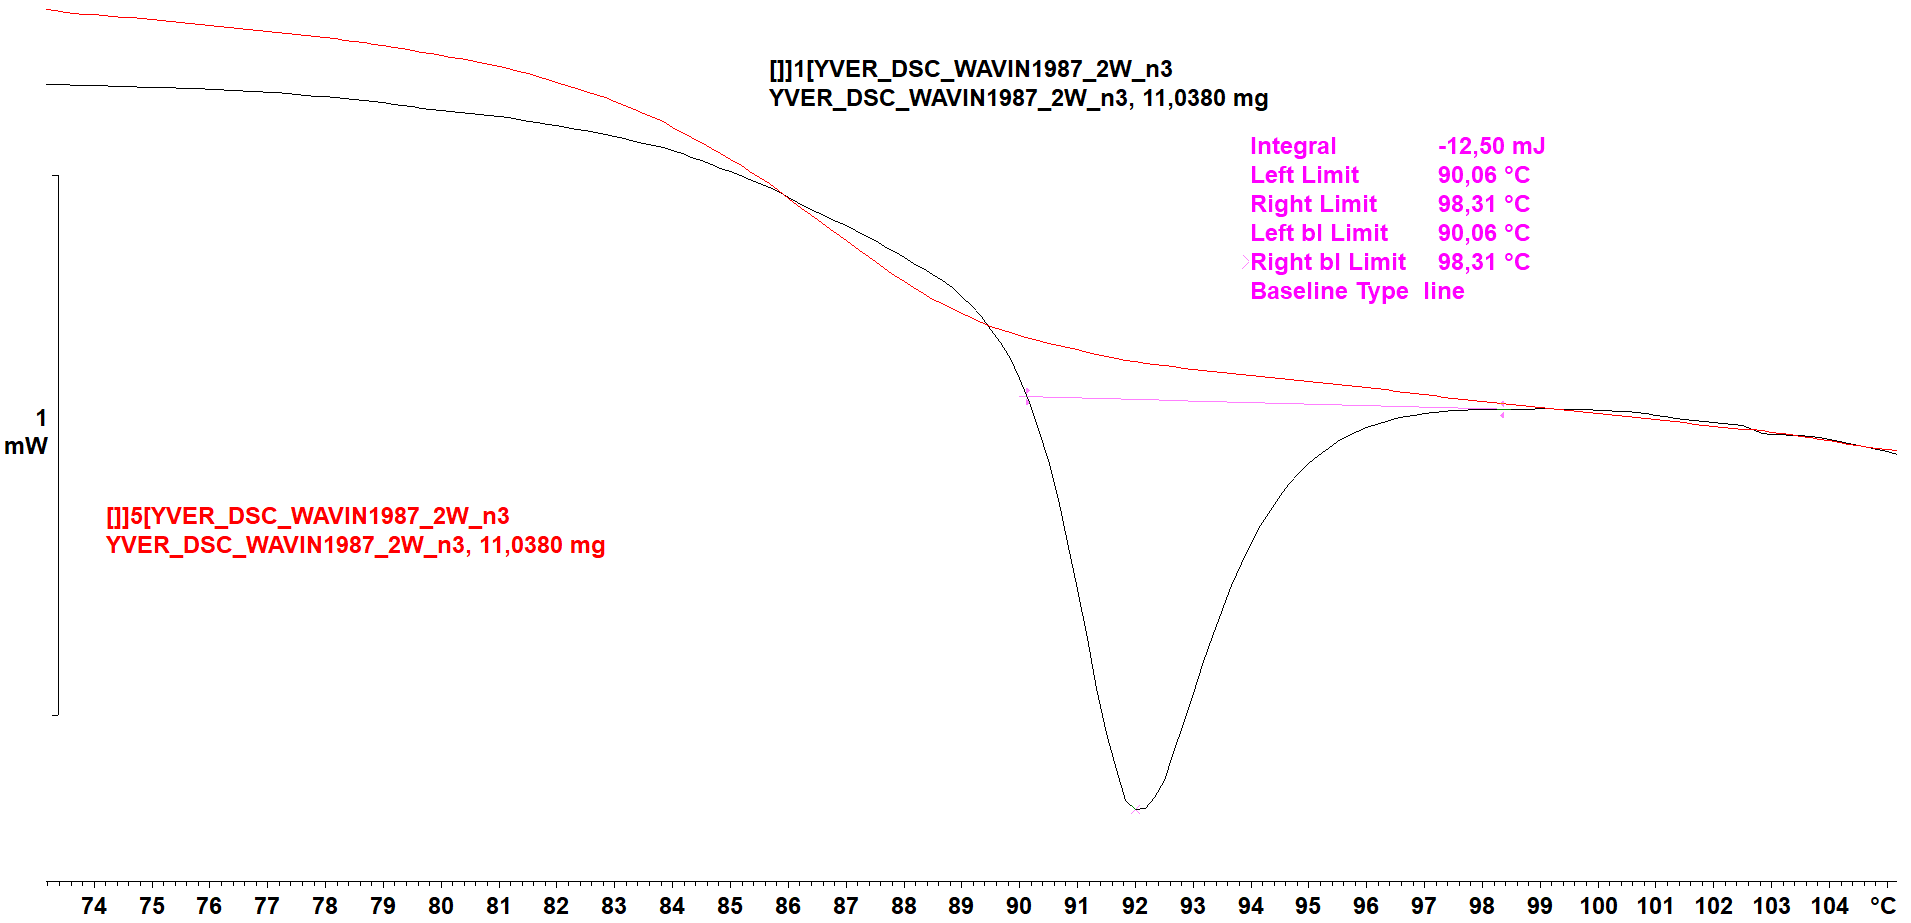
\includegraphics[width=0.75\linewidth]{Wavin1987_DSC_2w_n3.png}
    \caption{Endothermic peak of Wavin 1987, 2 weeks ageing, n°3}
    \label{fig:wavin1987_2w_n3}
\end{figure}
\begin{figure}[H]
    \centering
    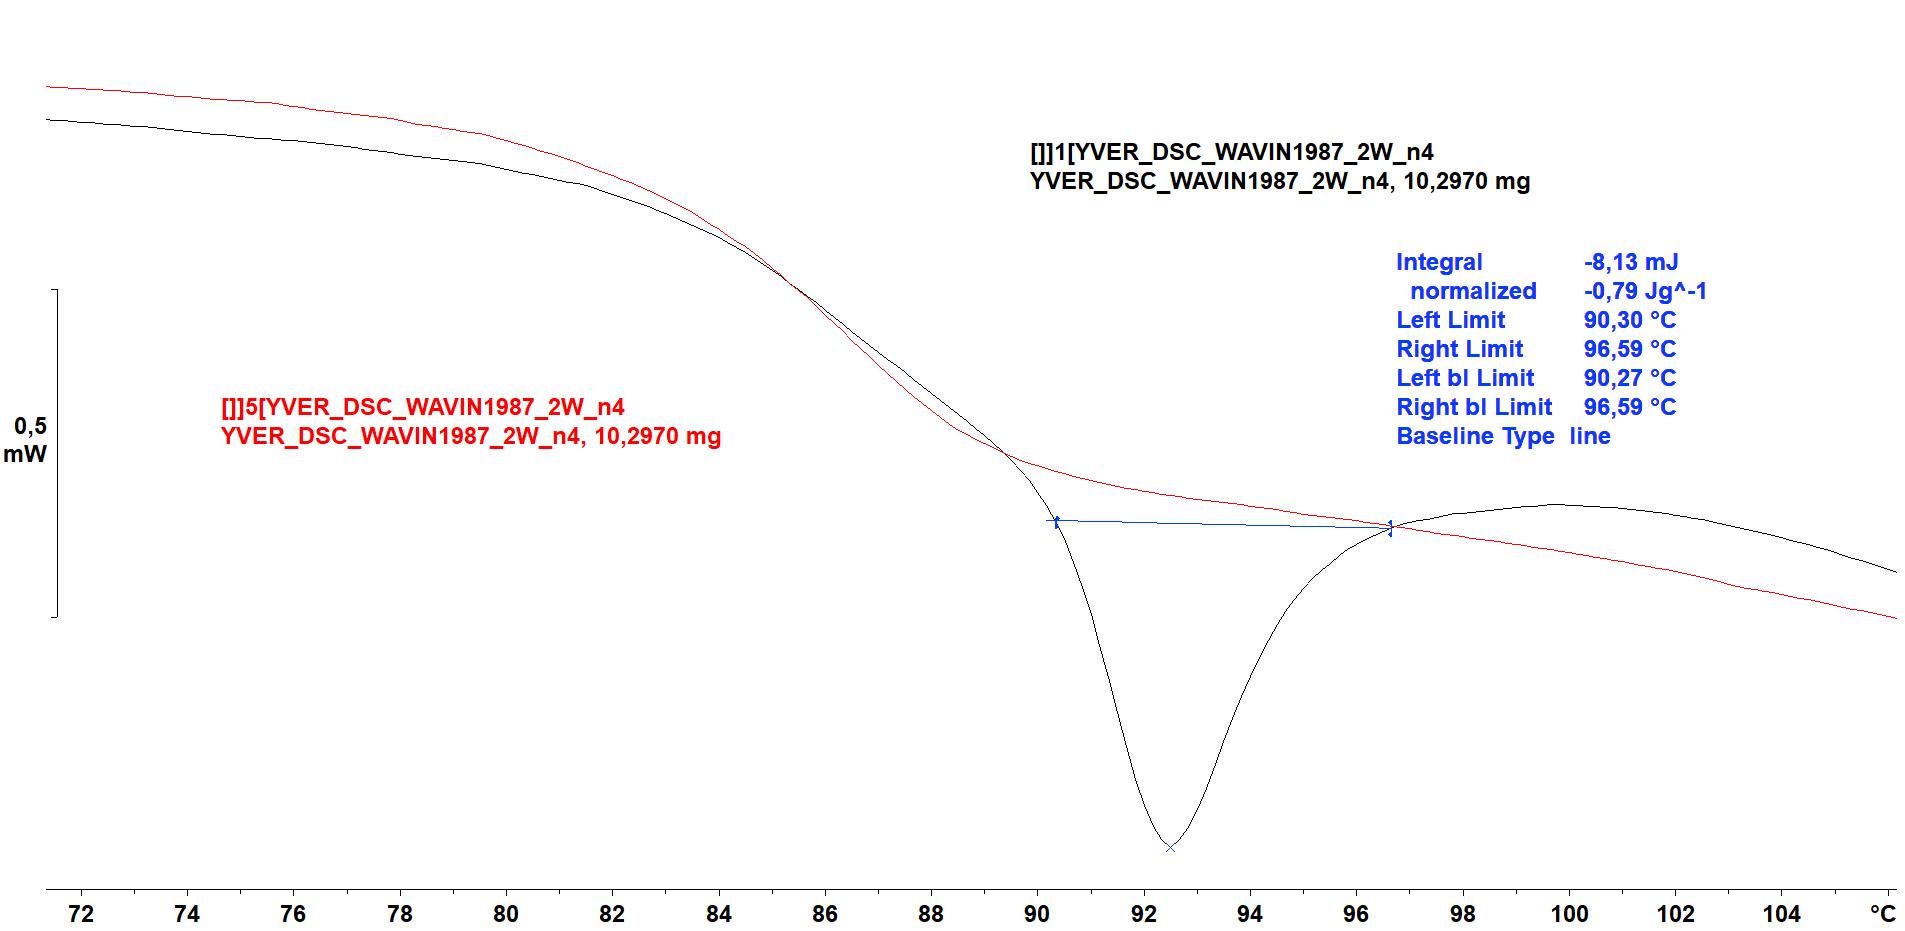
\includegraphics[width=0.75\linewidth]{Wavin1987_DSC_2w_n4.png}
    \caption{Endothermic peak of Wavin 1987, 2 weeks ageing, n°4}
    \label{fig:wavin1987_2w_n4}
\end{figure}

\section{Tensile tests}
Mechanical characterization was conducted at WAVIN through uniaxial tensile tests according to ISO 527. The objective was to monitor how ageing influences stiffness, yield behaviour, and failure mechanisms of uPVC.
Two configurations were used: one dedicated to accurate measurement of Young’s modulus at low strain, and one for complete tensile behaviour up to fracture.

\subsection{Young modulus test's parameters}
\begin{table}[h!]
\centering
\begin{tabular}{l l}
\hline
\textbf{Parameter} & \textbf{Value} \\
\hline
Customer & Wetsus \\
Test standard & ISO 527 \\
Material & uPVC \\
Specimen type & Type 1A -- IM at T\&I \\
Pre-load & 2 N \\
Test speed & 1 mm/min \\
Grip to grip separation at start & 115 mm \\
Machine data & 10 kN -- APP-354 -- clip on with Lo=75 mm; Wanddikte meter: 3-WDM-26 \\
\hline
\end{tabular}
\end{table}
\subsection{Tensile test's parameters}
\begin{table}[h!]
\centering
\begin{tabular}{l l}
\hline
\textbf{Parameters for tensile test} & \textbf{Value} \\
\hline
Customer & Wetsus \\
Test standard & ISO 527 \\
Material & uPVC \\
Specimen type & Type 1A \\
Pre-load & 5 lbf \\
Gage length for fine strain & 75 mm \\
Test speed & 5 mm/min \\
Grip to grip separation at start & 115 mm \\
Machine data & APP-354 \# 10 kN; Wanddikte meter: 3-WDM-26 \\
\hline
\end{tabular}
\end{table}

\subsection{Young moudulus through ageing}
\begin{figure}[H]
    \centering
    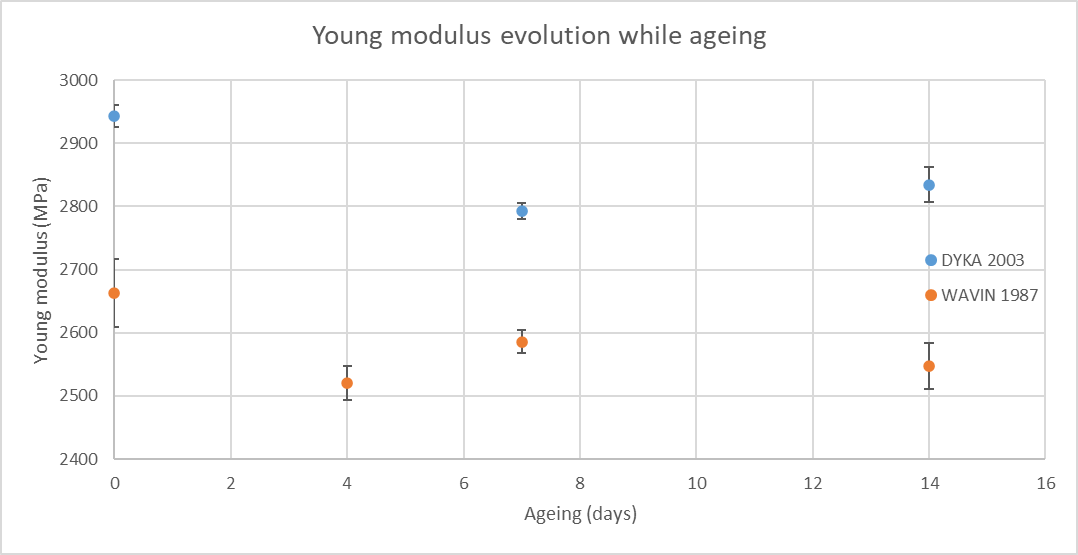
\includegraphics[width=0.75\linewidth]{evol_young_mod.png}
    \caption{Evolution of Young modulus}
    \label{fig:graph_young_mod_dyka_wavin}
\end{figure}
\subsection{Upper yield point}
\begin{figure}[H]
    \centering
    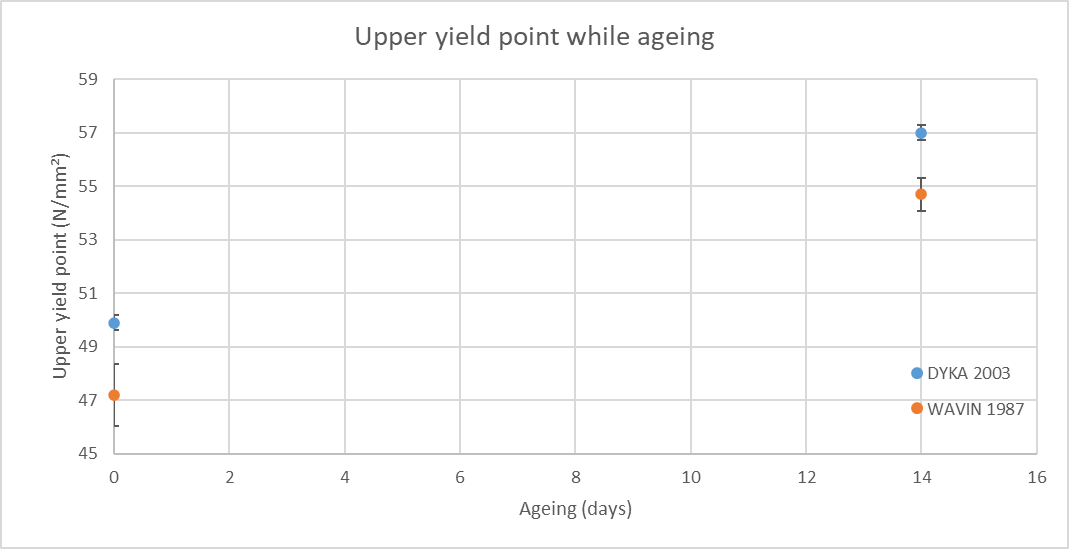
\includegraphics[width=0.75\linewidth]{evol_upper_yield.png}
    \caption{Evolution of the upper yield point}
    \label{fig:graph_upper_yield_dyka_wavin}
\end{figure}

\subsection{dL and force at break}
\begin{figure}[H]
    \centering
    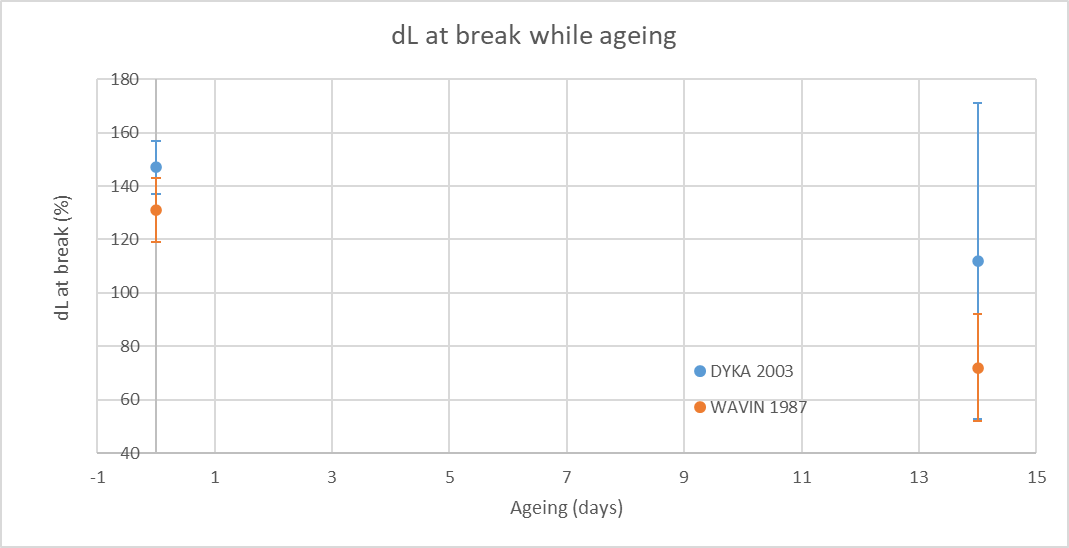
\includegraphics[width=0.75\linewidth]{evol_dL_break.png}
    \caption{Evolution of the dL at break}
    \label{fig:graph_dL_break_dyka_wavin}
\end{figure}
\begin{figure}[H]
    \centering
    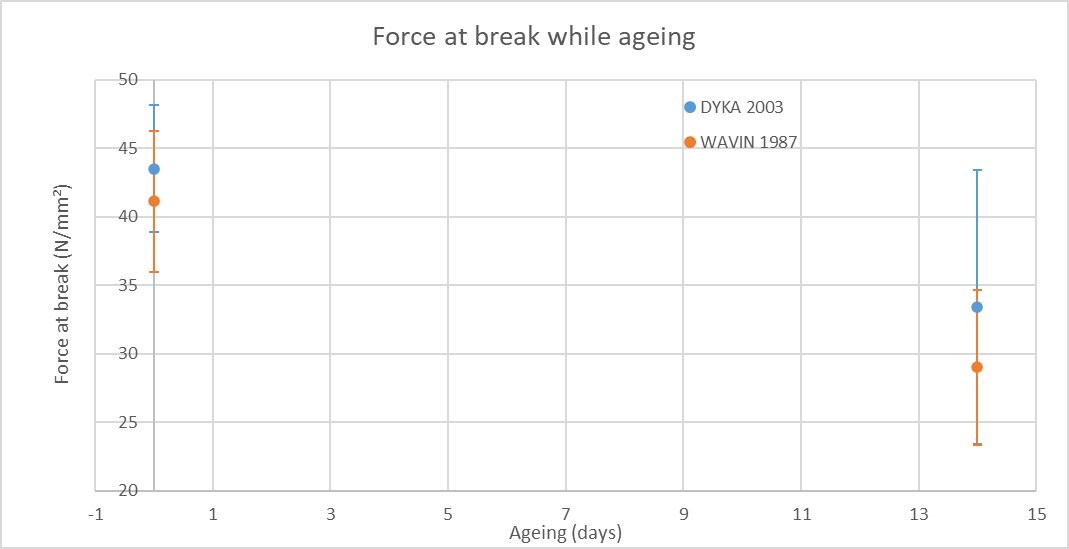
\includegraphics[width=0.75\linewidth]{evol_Fbreak.png}
    \caption{Evolution of the force at break}
    \label{fig:graph_force_break_dyka_wavin}
\end{figure}
\section{Wave mixing}

Nonlinear ultrasonic wave-mixing experiments were performed on a DYKA 2003 pipe and a WAVIN 1987 pipe with a thickness around 4.5 mm. The goal was to investigate the sensitivity of this non-destructive technique to changes in the material caused by aging.

The measurements were carried out using a phased array (PA) with elements 13 to 20, corresponding to pins 34, 24, 14, 4, 151, 141, 131, and 121. These elements were read out on channels 1 to 8, respectively. Two transducers, NDT and Harisonic, were initially inclined at 34° and -50° relative to the sample. The PVC front face was positioned approximately 89 mm from the rotational axes of the transducers and 71 mm from the PA. The transducers were spaced 305 mm apart, with a parallel ruler distance of 135 mm. The PA was initially centered at 240 mm, while the PVC sample extended from 180 mm to 290 mm along the measurement axis.

For excitation, channel 1 (NDT) sent a 30-cycle burst at 0.17 Vpp and 1,312,500 Hz, with a variable delay of 31.4413~µs. Channel 2 (Harisonic) sent a 40-cycle burst at 0.17 Vpp and 937,500 Hz. Each measurement location was sampled using four polarity configurations for the transducers: NORM/NORM, INV/NORM, INV/INV, and NORM/INV.

The TiePieScope oscilloscope recorded signals at a 20~MHz sampling frequency with 5000 samples, 14-bit resolution, and a 0.4~V range. Reference voltages were monitored simultaneously using a PicoScope with a sampling interval of $9.6 \times 10^{-8}$~s and a total duration of $8 \times 10^{-5}$~s.

The experiments were performed on 21/11/2025. The measurement positions were controlled with an XYZ table (X: -18 to 24~mm, step 2~mm; Y: 0, step 10~mm; Z: 34~mm, step 1~mm).




\begin{table}[h!]
\centering
\begin{tabular}{l c c c c c c}
\hline
\textbf{DYKA 2003} & & & & & & \\
\textbf{Test} & \textbf{Ageing (days)} & \textbf{Max amplitude (dBV)} &
\textbf{Max amplitude (µA)} & \textbf{Max noise floor (µA)} &
\textbf{R² Gaussian fit} & \textbf{Mean amplitude (dBV)} \\
\hline
n1 & 0  & -61.447 & 8.55e-04 & 9.97e-06 & 0.9933 & \multirow{3}{*}{-61.38533333} \\
n2 & 0  & -61.127 & 8.93e-04 & 9.85e-06 & 0.9926 & \\
n3 & 0  & -61.582 & 8.27e-04 & 9.82e-06 & 0.9939 & \\
\hline
n1 & 14 & -61.389 & 8.47e-04 & 1.01e-05 & 0.9931 & \multirow{3}{*}{-61.274} \\
n2 & 14 & -61.213 & 8.75e-04 & 1.13e-05 & 0.9921 & \\
n3 & 14 & -61.220 & 9.06e-04 & 1.05e-05 & 0.9839 & \\
\hline
\end{tabular}
\end{table}

\begin{table}[h!]
\centering
\begin{tabular}{l c c c c c c}
\hline
\textbf{WAVIN 1987} & & & & & & \\
\textbf{Test} & \textbf{Ageing (days)} & \textbf{Max amplitude (dBV)} & 
\textbf{Max amplitude (µA)} & \textbf{Max noise floor (µA)} &
\textbf{R² Gaussian fit} & \textbf{Mean amplitude (dBV)} \\
\hline
n8  & 0  & -63.027 & 7.14e-04 & 1.16e-05 & 0.9743 & \multirow{3}{*}{-62.816667} \\
n9  & 0  & -62.537 & 7.65e-04 & 1.04e-05 & 0.9783 & \\
n10 & 0  & -62.886 & 7.39e-04 & 1.12e-05 & 0.9756 & \\
\hline
n1  & 4  & -60.105 & 9.79e-04 & 1.18e-05 & 0.9955 & \multirow{3}{*}{-60.392} \\
n2  & 4  & -60.703 & 9.68e-04 & 1.08e-05 & 0.9964 & \\
n3  & 4  & -60.368 & 9.82e-04 & 1.06e-05 & 0.9907 & \\
\hline
n1  & 7  & -60.018 & 1.00e-03 & 1.13e-05 & 0.9969 & \multirow{3}{*}{-60.232} \\
n2  & 7  & -60.584 & 9.95e-04 & 1.16e-05 & 0.9944 & \\
n3  & 7  & -60.094 & 9.55e-04 & 1.22e-05 & 0.9956 & \\
\hline
n1  & 14 & -62.402 & 7.65e-04 & 1.14e-05 & 0.9897 & \multirow{3}{*}{-62.440333} \\
n2  & 14 & -62.373 & 7.71e-04 & 1.05e-05 & 0.9884 & \\
n3  & 14 & -62.546 & 7.71e-04 & 1.02e-05 & 0.9796 & \\
\hline
\end{tabular}
\end{table}

\begin{figure}[H]
    \centering
    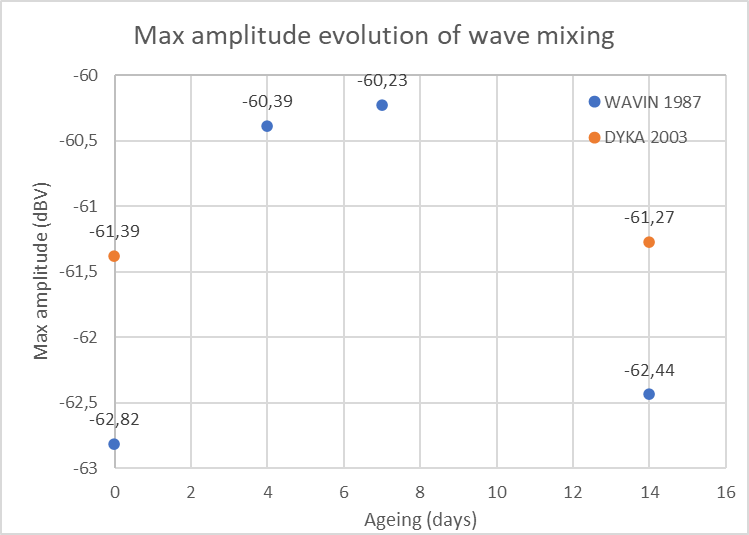
\includegraphics[width=0.75\linewidth]{max_amp_evol.png}
    \caption{Evolution of the maximum amplitude through ageing}
    \label{fig:graph_max_amp_dyka_wavin}
\end{figure}


\end{document}
